%Version 3.1 December 2024 -- Springer Nature LaTeX template (sn-jnl), adapted for this manuscript.
%
%%%%%%%%%%%%%%%%%%%%%%%%%%%%%%%%%%%%%%%%%%%%%%%%%%%%%%%%%%%%%%%%%%%%%%
%%                                                                 %%
%% Submit as one .tex document (no \input). Figures are attached   %%
%% separately (folder figures/). Bibliography: references.bib.     %%
%%                                                                 %%
%%%%%%%%%%%%%%%%%%%%%%%%%%%%%%%%%%%%%%%%%%%%%%%%%%%%%%%%%%%%%%%%%%%%%
%
% Lines marked "TODO(author)" must be completed by the authors before submission.

\documentclass[pdflatex,sn-mathphys-num]{sn-jnl}% Math and Physical Sciences Numbered Reference Style
%%\documentclass[pdflatex,sn-basic]{sn-jnl}% Basic Springer Nature Reference Style
%%\documentclass[lineno,pdflatex,sn-mathphys-num]{sn-jnl}% with line numbers for review

%%%% Standard Packages
\usepackage{graphicx}%
\usepackage{multirow}%
\usepackage{amsmath,amssymb,amsfonts}%
\usepackage{amsthm}%
\usepackage{mathrsfs}%
\usepackage[title]{appendix}%
\usepackage{xcolor}%
\usepackage{textcomp}%
\usepackage{manyfoot}%
\usepackage{booktabs}%
\usepackage{algorithm}%
\usepackage{algorithmicx}%
\usepackage{algpseudocode}%
\usepackage{listings}%
%%%% Additional packages
\usepackage{tikz}%
\usetikzlibrary{arrows.meta,positioning,fit,calc}%
%%%%

\theoremstyle{thmstyleone}%
\newtheorem{theorem}{Theorem}%
\newtheorem{proposition}[theorem]{Proposition}%
\theoremstyle{thmstyletwo}%
\newtheorem{example}{Example}%
\newtheorem{remark}{Remark}%
\theoremstyle{thmstylethree}%
\newtheorem{definition}{Definition}%

\newcommand{\kmsq}{km$^2$}
\newcommand{\kmsqa}{km$^2$\,a$^{-1}$}

\raggedbottom

\begin{document}

\title[Automated multi-temporal mapping of Chhota Shigri Glacier with GlaViTU]{Automated multi-temporal delineation and terminus retreat of Chhota Shigri Glacier, western Himalaya, from Sentinel-2 using a transferred convolutional-transformer model and calibrated self-training}

%%=============================================================%%
%% TODO(author): confirm names, order, affiliations and e-mail. %%
%%=============================================================%%
\author*[1]{\fnm{Sunny} \sur{Gupta}}\email{author@institution.edu}% TODO(author): corresponding e-mail

\affil*[1]{\orgdiv{Department}, \orgname{Institution}, \orgaddress{\city{City}, \postcode{000000}, \state{State}, \country{India}}}% TODO(author)

%%==================================%%
%% Unstructured abstract            %%
%%==================================%%
\abstract{Himalayan glacier outlines are still largely drawn by hand, which limits how often they can be updated. We test whether a published glacier-segmentation model can be transferred to one debris-affected glacier and used to quantify change without manual tracing. GlaViTU, a convolutional-transformer network, was applied to Sentinel-2 and Copernicus DEM data of Chhota Shigri Glacier (Himachal Pradesh, India) for 2017--2025. On 57 held-out High Mountain Asia benchmark tiles, regional fine-tuning raised the intersection over union from 0.678 to 0.748, and self-training on calibrated, multi-temporal pseudo-labels from independent years reached 0.779. The DEM was the most important input (+0.149), whereas Sentinel-1 backscatter gave no benefit. Isotonic calibration reduced the expected calibration error from 0.239 to 0.011, which made confidence-based pseudo-labelling possible. A per-pixel median over all clear scenes of each year reduced the between-scene area spread from about 1\,\kmsq\ to 0.3--0.8\,\kmsq; even so, no area trend is significant for any model. Terminus retreat over 2021--2025, however, is detected by all five models: 70--160\,m, or about 20--28\,m\,a$^{-1}$, concentrated within 1\,km of the terminus and on steep margins. Automated delineation can therefore monitor terminus change of a single Himalayan glacier, while area change remains limited by surface conditions on debris-covered margins.}

\keywords{Glacier mapping, Deep learning, Vision transformer, Sentinel-2, Self-training, Terminus retreat, Himalaya}

\maketitle

%%====================================================================%%
\section{Introduction}\label{sec1}
%%====================================================================%%

Himalayan glaciers supply water to some of the most densely populated river basins on Earth, and most of them are losing mass \cite{bolch2012,hugonnet2021}. Their retreat also creates and enlarges glacial lakes, which can fail as glacial lake outburst floods (GLOFs); High Mountain Asia has the largest population exposed to this hazard worldwide \cite{taylor2023}. Monitoring how individual glaciers change is therefore of both scientific and practical value.

Glacier outlines are the basis of this monitoring, but they are still mostly drawn or corrected by hand. Manual delineation is slow, depends on the analyst, and is especially uncertain on debris-covered tongues, where ice and rock look alike in optical images \cite{paul2013,scherler2011}. Global inventories such as the Randolph Glacier Inventory (RGI) \cite{rgi6,rgi7} and the GLIMS database \cite{raup2007} therefore describe each glacier at one date, and the outlines of a single glacier can differ by several square kilometres between analysts because of different ice divides.

Deep learning offers a way to automate this task. Convolutional networks have been used to map debris-covered glaciers from optical images and terrain data \cite{xie2020}, and the convolutional-transformer model GlaViTU recently reached expert-level accuracy on a global benchmark of glacier outlines \cite{maslov2025}. GlaViTU combines a transformer encoder \cite{dosovitskiy2021,zheng2021}, which captures context over a whole image patch, with a residual U-Net \cite{ronneberger2015,he2016}, which recovers sharp boundaries. Its accuracy is lowest, however, in debris-rich regions such as High Mountain Asia \cite{maslov2025}, and it has not been tested as a tool for measuring year-to-year change of a single glacier.

Two problems arise when such a model is used for change detection. First, a model that is accurate on average may not be stable from one image to the next, because surface conditions such as thin snow on debris change within days. Second, adapting the model to a new site normally needs labelled examples from that site, which would reintroduce manual tracing.

This study addresses both problems for Chhota Shigri Glacier, a benchmark glacier of the western Himalaya with a long field record \cite{wagnon2007,azam2016,mandal2020}. We ask whether a pretrained glacier-segmentation model can be transferred to the Himalaya and then delineate one glacier across years well enough to quantify retreat, without any manual outline. Specifically, we test (i) whether regional fine-tuning and site adaptation improve accuracy, (ii) which inputs matter, (iii) whether confidence-aware pseudo-labelling \cite{lee2013,xie2020noisy} can adapt the model without labels, and (iv) whether the resulting outlines are precise enough to detect change in area and terminus position over 2017--2025. To keep every result reproducible, all inputs are open data, every processing step is automatic, and the years used for training are separated from the years in which change is measured.

%%====================================================================%%
\section{Study area and data}\label{sec2}
%%====================================================================%%

\subsection{Study area}\label{subsec2.1}

Chhota Shigri Glacier lies in the Chandra valley of Lahaul, Himachal Pradesh, India (centroid 32.224\textdegree\,N, 77.508\textdegree\,E; Fig.~\ref{fig:study}). It is a valley glacier of about 15.5--15.7\,\kmsq\ \cite{wagnon2007,mandal2020}, extending from about 4050\,m to above 6000\,m~a.s.l., with a debris-covered tongue. It lies in the transition zone between the monsoon and the arid climate of the western Himalaya and has been monitored in the field since 2002 \cite{wagnon2007,azam2016}. Its mean annual glaciological mass balance was $-0.46 \pm 0.40$\,m\,w.e.\,a$^{-1}$ over 2002--2019 \cite{mandal2020}, and its terminus retreated by 800--850\,m between 1972 and 2009 \cite{gantayat2017}.

The glacier is identified as \texttt{RGI60-14.15990} in RGI~6.0 and \texttt{RGI2000-v7.0-G-14-30579} in RGI~7.0. All products were computed on one grid in UTM zone 43N with 10\,m pixels (1434 $\times$ 1254 pixels), snapped to the 60\,m Sentinel-2 tile lattice so that the 10, 20 and 60\,m bands align exactly with the grid. Glacier pixels are counted only inside a fixed analysis domain: the RGI~7.0 outline buffered by 1\,km, minus 33 neighbouring RGI~7.0 glaciers (47.9\,\kmsq). A fixed domain keeps the ice divides constant through time, so that area differences reflect changes of the margins and not of basin definitions; the seven GLIMS outlines of the glacier range from 11.6 to 16.8\,\kmsq, mostly because of different divides.

\begin{figure}[h]
\centering
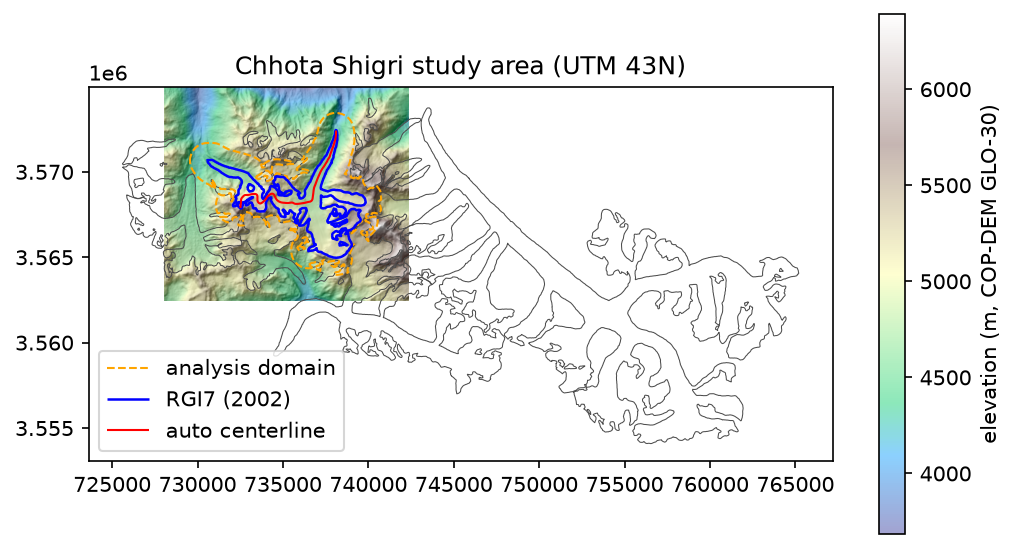
\includegraphics[width=0.85\textwidth]{figures/study_area.png}
\caption{Chhota Shigri study area in UTM zone 43N. Background: Copernicus GLO-30 elevation. Blue: RGI~7.0 outline (2002). Orange dashed: analysis domain (RGI~7.0 + 1\,km, minus neighbouring glaciers). Red: automatically derived centerline. Grey: neighbouring RGI~7.0 glaciers.}\label{fig:study}
\end{figure}

\subsection{Data}\label{subsec2.2}

Table~\ref{tab:data} lists all data sets. GlaViTU was trained on top-of-atmosphere (L1C) Sentinel-2 reflectance \cite{maslov2025,drusch2012}, so L1C was used as the model input. Scenes were discovered and screened with the Level-2A products and their scene classification layer (SCL) on Microsoft Planetary Computer \cite{planetarycomputer}, and the matching L1C products were read from the public Google Cloud archive. The labelled data for model training and testing are the High Mountain Asia (HMA) tiles of the GlaViTU benchmark \cite{maslov2024data}, read by HTTP byte-range requests from the 411\,GB archive. The official split of 165 training, 55 validation and 57 test tiles was kept, and no benchmark tile lies within 0.05\textdegree\ of the study site.

\begin{table}[h]
\caption{Data sets used in this study.}\label{tab:data}%
\begin{tabular}{@{}p{3.1cm}p{4.3cm}p{4.2cm}@{}}
\toprule
Data set & Content & Use \\
\midrule
Sentinel-2 L1C / L2A \cite{drusch2012} & Tile 43SGR, 15 Aug--15 Oct, 2017--2025 & Model input (L1C); scene screening (L2A SCL) \\
Copernicus DEM GLO-30 \cite{copdem} & Elevation, 30\,m & Model input (elevation, slope); analysis \\
Sentinel-1 RTC \cite{torres2012} & VV backscatter, ascending and descending & Model M3 only \\
RGI~6.0 / 7.0 \cite{rgi6,rgi7}, GLIMS \cite{raup2007} & Glacier outlines (2002 and older) & Domain, core, centerline; agreement test \\
GlaViTU benchmark, HMA \cite{maslov2024data} & 165 / 55 / 57 labelled tiles & Training, model selection, testing \\
GlaViTU weights \cite{maslov2025} & Global and HMA checkpoints & M0, M1 and initialisation \\
\botrule
\end{tabular}
\footnotetext{All data are openly available. No outline drawn in this study is used as input or label.}
\end{table}

%%====================================================================%%
\section{Methods}\label{sec3}
%%====================================================================%%

\subsection{Workflow overview}\label{subsec3.1}

Figure~\ref{fig:workflow} summarises the workflow. One script runs every step from data download to figures. The analysis epochs are the odd years 2017, 2019, 2021, 2023 and 2025. The even years 2018, 2020, 2022 and 2024 are used only to build pseudo-labels for the site-adapted model, so no model is trained on an image in which change is measured.

\begin{figure}[h]
\centering
\resizebox{\textwidth}{!}{%
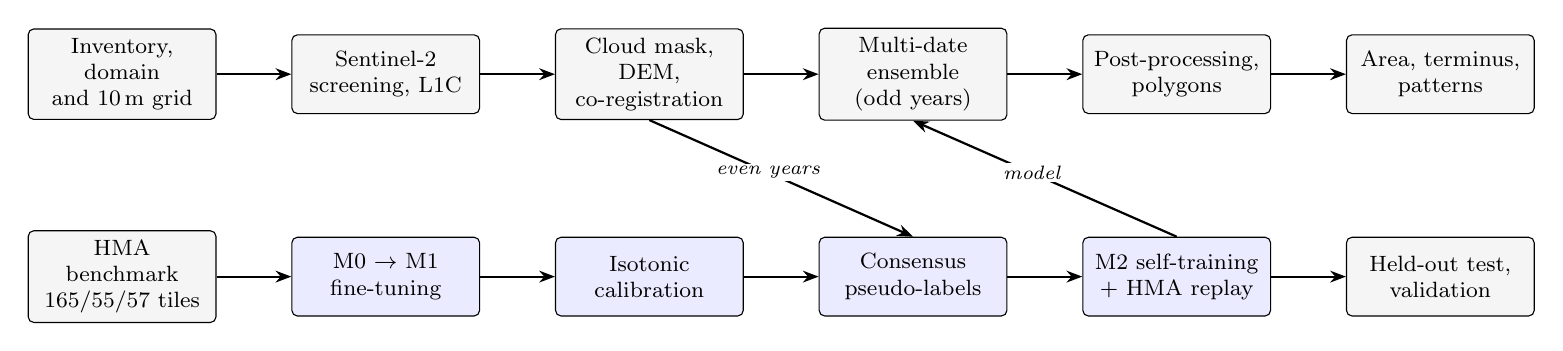
\begin{tikzpicture}[
  font=\footnotesize,
  box/.style={draw, rounded corners=2pt, align=center, minimum height=1.0cm, text width=2.15cm, fill=gray!8},
  hl/.style={box, fill=blue!8},
  arr/.style={-{Stealth[length=2mm]}, thick},
  lab/.style={font=\scriptsize\itshape, fill=white, inner sep=1pt},
  node distance=1.4cm and 0.95cm]
% row 1: site data and analysis
\node[box] (inv) {Inventory, domain\\and 10\,m grid};
\node[box, right=of inv] (s2) {Sentinel-2\\screening, L1C};
\node[box, right=of s2] (pre) {Cloud mask, DEM,\\co-registration};
\node[box, right=of pre] (ens) {Multi-date ensemble\\(odd years)};
\node[box, right=of ens] (post) {Post-processing,\\polygons};
\node[box, right=of post] (chg) {Area, terminus,\\patterns};
% row 2: models
\node[box, below=of inv] (bench) {HMA benchmark\\165/55/57 tiles};
\node[hl, right=of bench] (m1) {M0 $\rightarrow$ M1\\fine-tuning};
\node[hl, right=of m1] (cal) {Isotonic\\calibration};
\node[hl, right=of cal] (pl) {Consensus\\pseudo-labels};
\node[hl, right=of pl] (m2) {M2 self-training\\+ HMA replay};
\node[box, right=of m2] (test) {Held-out test,\\validation};
\draw[arr] (inv) -- (s2);
\draw[arr] (s2) -- (pre);
\draw[arr] (pre) -- (ens);
\draw[arr] (ens) -- (post);
\draw[arr] (post) -- (chg);
\draw[arr] (bench) -- (m1);
\draw[arr] (m1) -- (cal);
\draw[arr] (cal) -- (pl);
\draw[arr] (pl) -- (m2);
\draw[arr] (m2) -- (test);
\draw[arr] (pre.south) -- node[lab, pos=0.45] {even years} (pl.north);
\draw[arr] (m2.north) -- node[lab, pos=0.55] {model} (ens.south);
\end{tikzpicture}}%
\caption{Workflow. Grey: data preparation and analysis; blue: model training and adaptation. Calibrated pseudo-labels are built only from the even years; change is measured only in the odd years. All steps are automatic.}\label{fig:workflow}
\end{figure}

\subsection{Preprocessing}\label{subsec3.2}

\paragraph{Scene selection.} For each year, all Sentinel-2 L2A items of tile 43SGR between 15 August and 15 October were retrieved, keeping one item per datatake. Each scene passed three gates over the analysis domain: an SCL cloud fraction of at most 0.6 (a loose pre-screen, because SCL often classifies bright ice as cloud), an SCL snow fraction of at most 0.45 on the domain outside the glacier (an indicator of fresh snowfall that hides the margins), and an s2cloudless \cite{skakun2022} cloud fraction of at most 0.5. The model products use only the \emph{core window} 15 August--15 September of every year; later scenes serve only for gap filling and a sensitivity test.

\paragraph{Radiometry and bands.} The six bands used by GlaViTU were read from L1C over the grid window only: B2, B3, B4 and B8 at their native 10\,m, and B11 and B12 resampled bilinearly from 20\,m. Digital numbers were converted to reflectance as $\rho = (\mathrm{DN} + \mathrm{offset})/Q$, with the radiometric offset and quantification value read from each product's metadata. This removes the $-1000$\,DN offset introduced by processing baseline 04.00 in 2022.

\paragraph{Clouds.} Cloud probability was computed with s2cloudless on ten L1C bands at 20\,m (threshold 0.4, 4-pixel averaging, 2-pixel or 40\,m dilation). Cloudy pixels were not removed from the image; their predictions were set to missing values after inference (Sect.~\ref{subsec3.7}).

\paragraph{Terrain.} Elevation was resampled bilinearly from the Copernicus GLO-30 DEM to 10\,m. Slope was computed with Horn's method \cite{horn1981} on a 30\,m version of the grid, close to the native DEM resolution, and resampled to 10\,m; this avoids artefacts of computing slope on an interpolated surface.

\paragraph{Co-registration.} Every analysis scene was aligned with the reference scene of 11 September 2023 by phase cross-correlation with 20$\times$ up-sampling \cite{guizar2008}, applied to Sobel gradients of band B8 in 256-pixel windows. Only stable terrain was used: outside the domain plus 300\,m, outside all glaciers plus 150\,m, slope below 35\textdegree, and cloud- and snow-free in both scenes (normalised difference snow index $<0.2$). Scenes with a median shift above 0.25\,pixel were corrected by a Fourier shift. Two scenes were corrected (0.67 to 0.11\,pixel and 0.36 to 0.14\,pixel), and all residuals are at most 1.6\,m.

\paragraph{Normalisation.} Inputs were min--max scaled with the official GlaViTU statistics of the global benchmark, separately for each band, elevation and slope. Statistics computed from the site would shift every input and degrade the pretrained weights.

\subsection{GlaViTU architecture}\label{subsec3.3}

GlaViTU \cite{maslov2025} has about 10 million parameters and takes 384 $\times$ 384 pixel patches (Fig.~\ref{fig:arch}). It has four stages.

\emph{Fusion block.} Each input group (optical: six bands; DEM: elevation and slope; SAR: two channels) passes through its own branch of two 3$\times$3 convolutions with batch normalisation and leaky ReLU, followed by a squeeze-and-excitation gate \cite{hu2018} that weights the 64 feature channels. The branch outputs are added, which allows input groups to be added or removed.

\emph{Transformer encoder.} The fused features are cut into 16 $\times$ 16 pixel tokens (a 24 $\times$ 24 grid of 160\,m squares), embedded to 64 dimensions with learned positional embeddings, and passed through 12 pre-norm transformer blocks with four-head self-attention and a 256-unit MLP \cite{dosovitskiy2021}. A progressive up-sampling decoder in the style of SETR \cite{zheng2021} restores full resolution, and the fusion features are added back. Self-attention lets each token use information from the whole 3.84\,km patch, for example the connection of a debris-covered tongue to the clean ice above it.

\emph{Residual U-Net.} A three-level residual U-Net \cite{ronneberger2015,he2016} (64--512 channels) refines the result at 10\,m resolution; its output is added to its input, so that it learns a correction to the transformer map.

\emph{Outputs.} A per-pixel softmax gives $P(\mathrm{glacier})$. A second softmax head after the transformer stage provides deep supervision during training only.

\begin{figure}[h]
\centering
\resizebox{0.98\textwidth}{!}{%
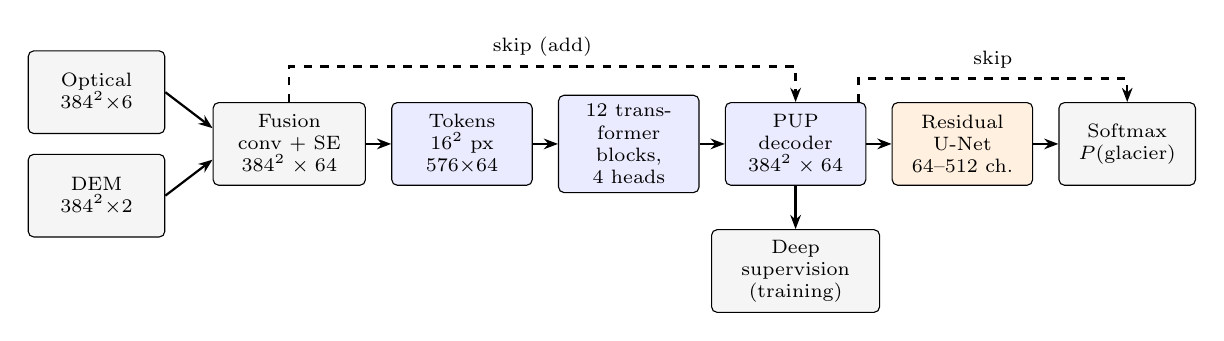
\begin{tikzpicture}[
  font=\scriptsize,
  blk/.style={draw, rounded corners=2pt, align=center, minimum height=1.05cm, text width=1.55cm, fill=gray!8},
  tr/.style={blk, fill=blue!8},
  un/.style={blk, fill=orange!12},
  arr/.style={-{Stealth[length=1.8mm]}, thick},
  node distance=0.32cm]
\node[blk, text width=1.5cm] (opt) {Optical\\$384^2{\times}6$};
\node[blk, text width=1.5cm, below=0.25cm of opt] (dem) {DEM\\$384^2{\times}2$};
\node[blk, text width=1.7cm, anchor=west] (fus) at ($(opt.east)!0.5!(dem.east)+(0.6,0)$) {Fusion\\conv + SE\\$384^2\times64$};
\node[tr, right=of fus] (tok) {Tokens\\$16^2$ px\\$576{\times}64$};
\node[tr, right=of tok] (enc) {12 transformer\\blocks, 4 heads};
\node[tr, right=of enc] (dec) {PUP decoder\\$384^2\times64$};
\node[un, right=of dec] (unet) {Residual\\U-Net\\64--512 ch.};
\node[blk, right=of unet, text width=1.5cm] (out) {Softmax\\$P$(glacier)};
\node[blk, below=0.55cm of dec, text width=1.9cm] (ds) {Deep\\supervision\\(training)};
\draw[arr] (opt.east) -- ([yshift=2mm]fus.west);
\draw[arr] (dem.east) -- ([yshift=-2mm]fus.west);
\draw[arr] (fus) -- (tok);
\draw[arr] (tok) -- (enc);
\draw[arr] (enc) -- (dec);
\draw[arr] (dec) -- (unet);
\draw[arr] (unet) -- (out);
\draw[arr] (dec) -- (ds);
\draw[arr, dashed] (fus.north) -- ++(0,0.45) -| node[pos=0.25, above] {skip (add)} (dec.north);
\draw[arr, dashed] (dec.north east) ++(-0.1,0) -- ++(0,0.3) -| node[pos=0.25, above] {skip} (out.north);
\end{tikzpicture}}%
\caption{GlaViTU architecture \cite{maslov2025} as used here. Grey: input-specific fusion with squeeze-and-excitation (SE); blue: transformer encoder with progressive up-sampling (PUP) decoder; orange: residual U-Net refinement. The deep-supervision head is used only in training. Model M3 adds a third fusion branch for Sentinel-1 backscatter.}\label{fig:arch}
\end{figure}

\subsection{Transfer-learning hierarchy}\label{subsec3.4}

Five main models and two ablation models share this architecture (Table~\ref{tab:models}). M0 is the published global model. M1 is the published fine-tuning of M0 on HMA tiles; M1-local is our reproduction of that recipe with a reduced budget. M2 starts from M1 and is adapted to Chhota Shigri by self-training (Sect.~\ref{subsec3.6}). M3 adds a Sentinel-1 branch, initialised randomly while all other layers are copied from M0. For a fair input ablation, M3, an optical + DEM model and an optical-only model were trained on the same 66 HMA tiles that contain SAR, with the same budget.

All fine-tuning reused the official GlaViTU data loader, augmentations (flips, rotation, crop-and-scale, gamma correction 0.8--1.2, group-wise feature occlusion, Gaussian shift and noise) and loss. The loss is the focal loss \cite{lin2017}
\begin{equation}
\mathcal{L}_\mathrm{focal} = -\sum_{c} y_c\,(1-p_c)^{\gamma}\log p_c, \qquad \gamma = 2,\label{eq:focal}
\end{equation}
applied to both heads with weights 0.5 (deep supervision) and 1.0 (output), with label smoothing of 0.1 \cite{szegedy2016}. Optimisation used Adam with cosine learning-rate decay, and the checkpoint with the best glacier IoU on the HMA validation tiles was kept. Only the budget was reduced: M1-local used 8 epochs of 250 steps (batch 4, learning rate $5\times10^{-5}$), about 1.7\,\% of the official number of steps; M2 used 4 epochs of 200 steps (learning rate $2\times10^{-5}$); the SAR-subset models used 4 epochs of 250 steps.

\begin{table}[h]
\caption{Model variants. All use the GlaViTU architecture.}\label{tab:models}%
\begin{tabular}{@{}p{2.3cm}p{1.6cm}p{2.9cm}p{2.1cm}p{2.3cm}@{}}
\toprule
Model & Learning & Labels & Initialised from & Inputs \\
\midrule
M0 global & Supervised\footnotemark[1] & Expert, worldwide & -- & Optical + DEM \\
M1 HMA official & Supervised\footnotemark[1] & Expert, HMA & M0 & Optical + DEM \\
M1-local & Supervised & Expert, 165 HMA tiles & M0 & Optical + DEM \\
M2 Chhota Shigri & Self-training & Pseudo-labels + HMA replay & M1 & Optical + DEM \\
M3 SAR & Supervised & Expert, 66 HMA tiles & M0 + new branch & Optical + DEM + SAR \\
Optical + DEM (abl.) & Supervised & Expert, 66 HMA tiles & M0 & Optical + DEM \\
Optical only (abl.) & Supervised & Expert, 66 HMA tiles & M0 & Optical \\
\botrule
\end{tabular}
\footnotetext{Optical: B2, B3, B4, B8, B11, B12; DEM: elevation and slope; SAR: Sentinel-1 VV ascending and descending.}
\footnotetext[1]{Published weights \cite{maslov2025}; not retrained in this study.}
\end{table}

\subsection{Probability calibration}\label{subsec3.5}

Label smoothing and the focal loss compress the softmax output: on the HMA validation tiles, the raw $P(\mathrm{glacier})$ of M1 lies only between 0.24 and 0.89. A confidence threshold such as 0.95 is therefore never reached. We calibrated each model by isotonic regression \cite{zadrozny2002}, a non-decreasing step function $g$ fitted to map raw probability to the observed glacier frequency. The monotonic constraint preserves the ranking of pixels, so outlines at a fixed threshold are not degraded. For M1, $g$ was fitted on 400\,000 pixels from 20 HMA validation tiles (ten tiles for the other models), and evaluated on a held-out half of the tiles by the expected calibration error \cite{naeini2015,guo2017}
\begin{equation}
\mathrm{ECE} = \sum_{b=1}^{B} \frac{n_b}{N}\,\bigl|\,\bar{p}_b - \bar{y}_b\,\bigr|, \qquad B = 15,\label{eq:ece}
\end{equation}
where $\bar{p}_b$ is the mean predicted probability and $\bar{y}_b$ the observed glacier fraction of the $n_b$ pixels in bin $b$. No site data enter the calibration.

\subsection{Calibrated multi-temporal pseudo-labels and self-training}\label{subsec3.6}

No outline of Chhota Shigri was drawn for training. Instead, the teacher M1 labelled the site, and only pixels on which it was confident and consistent across scenes and years were kept (Algorithm~\ref{alg:pl}). The teacher was applied to the core-window scenes of the even years (2018: 3 scenes, 2020: 4, 2022: 5, 2024: 3, of which one, 31 August 2024, contained no valid data). Thresholds act on calibrated probabilities. All other pixels, including every pixel that changes between years or flips with surface conditions, are left unlabelled. The labels therefore contain no assumption about the amount or direction of change. No inventory outline was used as a label.

\begin{algorithm}
\caption{Consensus pseudo-label for pixel $i$ (thresholds $\tau_g = 0.95$, $\tau_b = 0.05$, $f = 0.6$, $k = 3$)}\label{alg:pl}
\begin{algorithmic}[1]
\Require calibrated probabilities $p_{i,s}$ for the clear scenes $s$ of the training years $y \in Y$, $|Y| = 4$
\State $n \gets$ number of clear scenes of pixel $i$; $\tilde{p}_{i,y} \gets \mathrm{median}_{s \in y}\, p_{i,s}$
\If{$n \geq 3$ \textbf{and} $\#\{s : p_{i,s} \geq \tau_g\} \geq f\,n$ \textbf{and} $\min_s p_{i,s} > \tau_b$ \textbf{and} $\#\{y : \tilde{p}_{i,y} \geq \tau_g\} \geq k$}
  \State label$_i \gets$ glacier
\ElsIf{$n \geq 3$ \textbf{and} $\#\{s : p_{i,s} \leq \tau_b\} \geq f\,n$ \textbf{and} $\max_s p_{i,s} < \tau_g$ \textbf{and} $\#\{y : \tilde{p}_{i,y} \leq \tau_b\} \geq k$}
  \State label$_i \gets$ background
\Else
  \State label$_i \gets$ ignored \Comment{target $[0,0]$: zero focal loss}
\EndIf
\end{algorithmic}
\end{algorithm}

The consensus label map was attached to the image of \emph{every} training scene. A margin pixel that is confidently glacier in most scenes is thus also presented as glacier in a scene where it is snow-dusted, which teaches the student to ignore one-day surface conditions. Pixels that are cloudy in a scene carry no label in that scene. Each site scene was included twice, and 40 HMA training tiles were mixed in as replay to prevent forgetting of the expert labels. Label smoothing was applied only to labelled pixels. The M2 checkpoint was selected on the HMA validation tiles, never on site data.

\subsection{Multi-date ensemble and post-processing}\label{subsec3.7}

For each analysis year, every clear core-window scene was predicted with 384-pixel patches, a stride of 192 pixels and Gaussian-weighted blending. Cloudy pixels were set to missing, and the yearly probability map is the per-pixel median over scenes. A whole scene $j$ was rejected when its glacier area $A_j$ departed from the median $\tilde{A}$ by
\begin{equation}
|A_j - \tilde{A}| > \max\bigl(3 \times 1.4826\,\mathrm{MAD}(A),\; 0.5\,\mathrm{km}^2\bigr).\label{eq:outlier}
\end{equation}
Pixels without a clear core-window observation were filled from clear scenes of the same year outside the window; pixels still unobserved were reported. Post-processing applied a threshold of 0.5, a 3$\times$3 median filter, clipping to the domain, retention of 8-connected components that intersect the RGI~7.0 \emph{core} (the outline eroded by 300\,m), removal of objects below 100 pixels and filling of holes below 50 pixels, followed by polygonisation and validity checks. The core only identifies which ice body is Chhota Shigri; margins and terminus are entirely model-derived.

\subsection{Change quantification}\label{subsec3.8}

\paragraph{Area uncertainty.} The uncertainty of the area $A$ of each epoch combines three terms:
\begin{equation}
\sigma_A = \sqrt{\sigma_\mathrm{buf}^2 + \sigma_\mathrm{thr}^2 + \sigma_\mathrm{surf}^2},\label{eq:sigmaA}
\end{equation}
where $\sigma_\mathrm{buf}$ is half a pixel times the perimeter \cite{granshaw2006}, $\sigma_\mathrm{thr}$ is half the area difference between calibrated thresholds 0.4 and 0.6, and $\sigma_\mathrm{surf}$ is the standard deviation of the single-scene areas of the year. For a change relative to a baseline epoch 0, the buffer and surface terms of both epochs are combined in quadrature, while the threshold term is treated as systematic and recomputed on the difference:
\begin{equation}
\sigma_{\Delta A} = \sqrt{\sigma_{\mathrm{buf},t}^2 + \sigma_{\mathrm{buf},0}^2 + \sigma_{\mathrm{surf},t}^2 + \sigma_{\mathrm{surf},0}^2 + \sigma_{\Delta,\mathrm{thr}}^2}.\label{eq:sigmadA}
\end{equation}
Area trends were fitted by weighted least squares with weights $1/(\sigma_\mathrm{buf}^2 + \sigma_\mathrm{surf}^2)$.

\paragraph{Terminus.} A main centerline was generated automatically as a least-cost path from the terminus to the highest head within the RGI~7.0 outline, following Kienholz et al.\ \cite{kienholz2014}, with cost
\begin{equation}
c = 1 + 200\left(\frac{D_\mathrm{max} - D}{D_\mathrm{max}}\right)^{4},\label{eq:cost}
\end{equation}
where $D$ is the distance to the glacier margin. Terminus position was measured in two ways: as the most downstream centerline point reached continuously from the head, and by the box method, i.e.\ the glacier area inside a 2\,km $\times$ 159\,m box along the lowest part of the centerline divided by the box width. The uncertainty of each position is $\sigma_T = \sqrt{r^2 + e^2}$, with pixel size $r = 10$\,m and co-registration residual $e$, combined in quadrature for differences. Structural uncertainty is expressed by the spread across the five models.

\paragraph{Year of loss.} A pixel was assigned a loss year only if it was glacier in the baseline and non-glacier in that and every later epoch; pixels that were lost and re-appeared are reported as unstable.

\subsection{Spatial pattern analysis}\label{subsec3.9}

Persistent loss was compared with the retained baseline ice by 100\,m elevation band, slope class, aspect sector and distance to the terminus, as a loss fraction and as an enrichment (share of loss divided by share of baseline area). Hotspots were mapped with the Getis--Ord $G_i^*$ statistic \cite{getis1992,ord1995} on 100\,m cells with a 5$\times$5-cell neighbourhood, and a descriptive logistic model of loss against terrain was evaluated by five-fold spatial-block cross-validation with 1\,km blocks \cite{roberts2017}. These analyses describe where change occurred and are not forecasts.

\subsection{Validation strategy}\label{subsec3.10}

No contemporaneous independent outline of Chhota Shigri exists, so validation uses four complementary tests, none of which evaluates a model on its own labels: (A) pooled IoU on the 57 held-out HMA test tiles, with 95\,\% confidence intervals from a paired bootstrap over tiles; (B) agreement with the 2002 RGI~7.0 outline, for the whole glacier and for the zone above 5000\,m where little margin change is expected; (C) comparison with published areas and retreat rates \cite{wagnon2007,mandal2020,gantayat2017}; and (D) temporal consistency. Agreement in (B) measures consistency with an older outline, not accuracy.

\subsection{Error sources}\label{subsec3.11}

The satellite images are never edited. Each error source is handled by rejecting data, by the classification of the model, by temporal aggregation or by post-processing (Table~\ref{tab:errors}). Three sources are only partly handled or not handled: cloud shadow and terrain shadow have no explicit per-pixel mask, and there is no water mask.

\begin{sidewaystable}
\caption{Error sources in automated multi-temporal delineation, their handling and the remaining effect.}\label{tab:errors}
\begin{tabular*}{\textheight}{@{\extracolsep\fill}p{2.4cm}p{3.0cm}p{6.2cm}p{4.6cm}c}
\toprule
Error source & Mitigation (stage) & Implementation & Remaining effect & Status\footnotemark[1] \\
\midrule
Cloud & Scene rejection; per-pixel masking & s2cloudless $p \ge 0.4$, 40\,m dilation; scene rejected if domain cloud $> 0.5$; cloudy pixels set to missing before the median & Gaps filled from the same year & $\bullet$ \\
Cloud shadow & Indirect & Cloud-mask dilation; median and scene-outlier rejection & Not quantified & $\circ\!\bullet$ \\
Seasonal and fresh snow & Window; snow screening & 15 Aug--15 Sep in every year; scene rejected if SCL snow $> 45\,\%$ off-glacier & Later scenes map 1.5--4.6\,\kmsq\ less glacier & $\bullet$ \\
Thin snow on debris margins & Multi-date median; unlabelled in self-training & Per-pixel median over clear scenes; 34.7\,\% of pixels unlabelled & Spread $\approx 1$\,\kmsq\ reduced to 0.3--0.8\,\kmsq & $\circ\!\bullet$ \\
Debris-covered ice & Inputs; regional fine-tuning & Elevation and slope; transformer context; HMA training & DEM: $+0.149$ IoU; terminus position spread up to $\sim$800\,m & $\circ\!\bullet$ \\
Bare rock & Model; object filter & SWIR bands and DEM; objects $< 100$\,px removed, holes $< 50$\,px filled & Included in benchmark IoU & $\bullet$ \\
Proglacial water & None & -- & Not quantified & $\circ$ \\
Terrain shadow & Indirect & Window before low sun; slope input; median & Not quantified & $\circ\!\bullet$ \\
Seasonal timing & Fixed window & Same calendar window in every year & 2025 scenes from August only & $\circ\!\bullet$ \\
Misregistration & Co-registration & Phase correlation on stable terrain; shifts $> 0.25$\,px corrected & Residual $\le 1.6$\,m (analysis epochs) & $\bullet$ \\
Radiometric offset & Harmonisation & Per-product offset and quantification value & None expected & $\bullet$ \\
Anomalous scenes & Outlier rejection & Eq.~(\ref{eq:outlier}) & Logged per model and year & $\bullet$ \\
Data gaps & Same-year gap filling & No mixing of years; unobserved pixels reported & $\approx 3$\,\kmsq\ seen once in 2017 and 2019 & $\circ\!\bullet$ \\
Neighbouring glaciers & Domain; connectivity & Domain minus 33 glaciers; components touching the 300\,m core & Margins model-derived & $\bullet$ \\
Classification noise & Morphological filtering & 3$\times$3 median; slivers $< 4$\,px removed; validity checks & In $\sigma_\mathrm{buf}$ & $\bullet$ \\
\botrule
\end{tabular*}
\footnotetext[1]{$\bullet$ addressed explicitly; $\circ\!\bullet$ partly or indirectly addressed; $\circ$ not addressed.}
\end{sidewaystable}

\subsection{Experimental setup}\label{subsec3.12}

Training ran on an Apple M4 (16\,GB) with Python 3.11, TensorFlow 2.15.1 and tensorflow-metal 1.1.0, with a random seed of 42; a retry-and-resume wrapper handled intermittent GPU errors. Inference ran on the CPU (about 30\,s per scene) because model prediction on the GPU failed on real inputs. The GlaViTU code was fixed at commit \texttt{8c4eead} of the authors' repository, and the published weights were verified by checksums.

%%====================================================================%%
\section{Results}\label{sec4}
%%====================================================================%%

\subsection{Training behaviour}\label{subsec4.1}

Figure~\ref{fig:training} shows the training loss and the validation glacier IoU of the runs trained in this study. M1-local improved over the first six epochs and then levelled off. M2 started from a high validation IoU, inherited from M1, and kept it during self-training, which shows that the site adaptation did not degrade performance on the regional validation tiles. The optical-only model stayed far below all models with a DEM. The training loss of M2 is lower than that of the other runs because a third of the site pixels carry no loss and the labelled pixels are, by construction, the confident ones.

\begin{figure}[h]
\centering
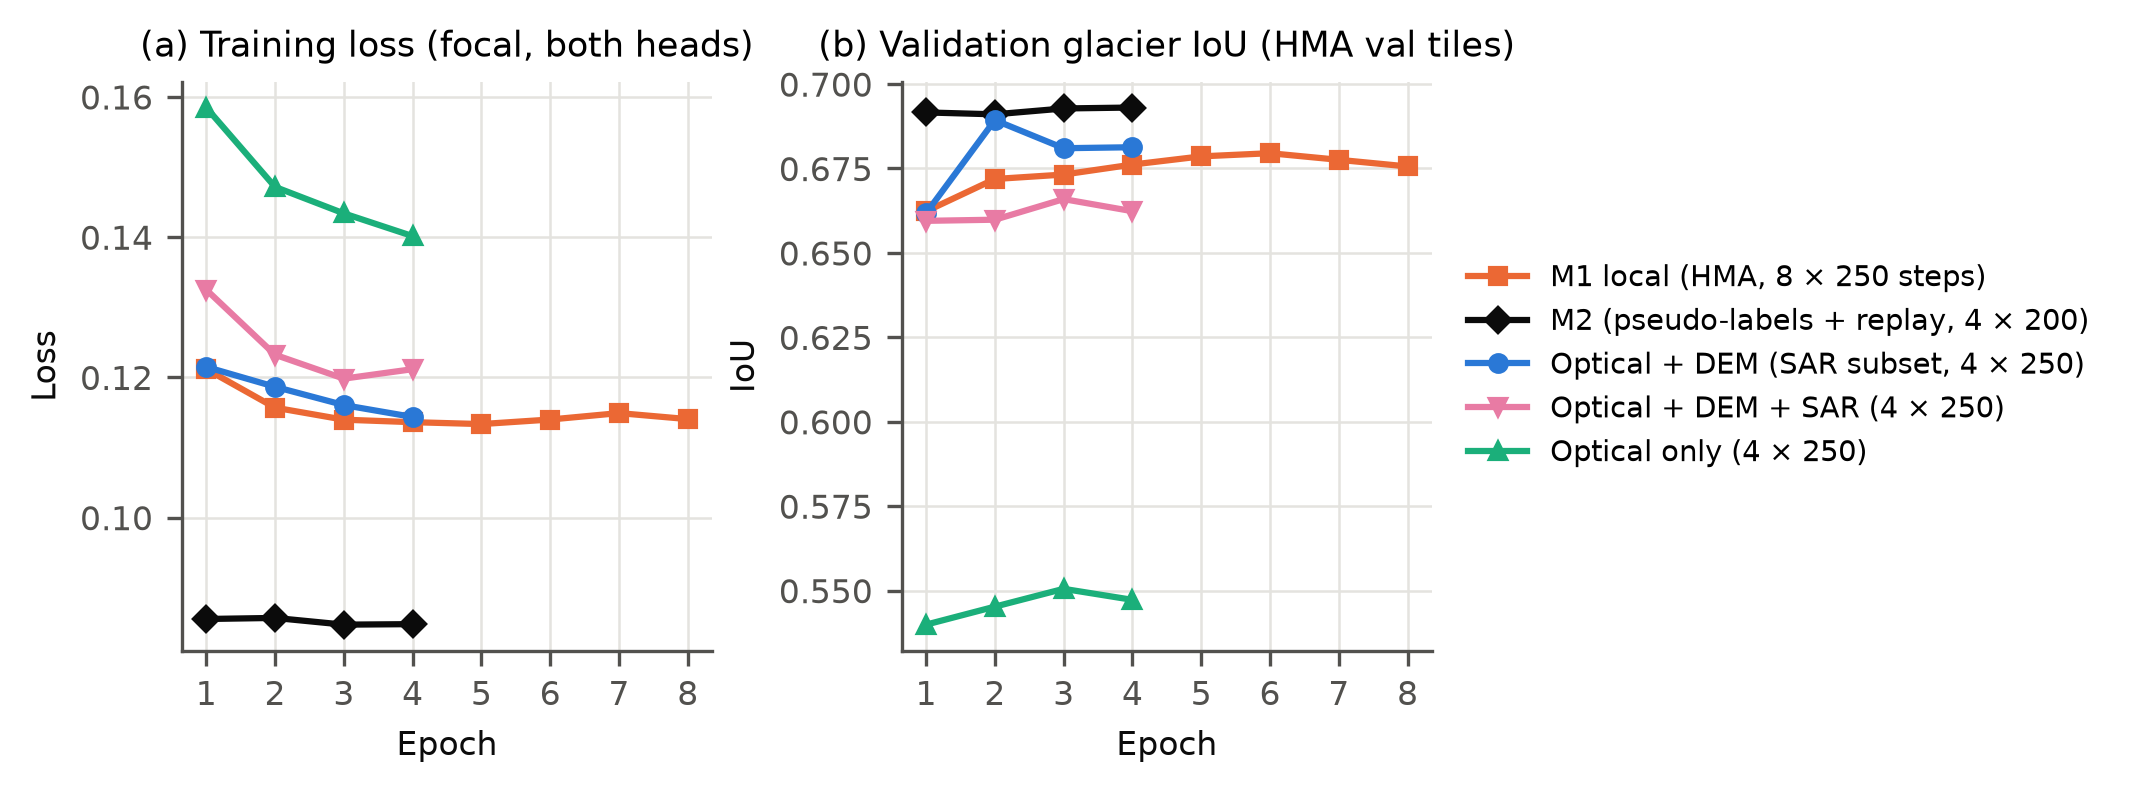
\includegraphics[width=\textwidth]{figures/fig_training.png}
\caption{Training curves of the models trained in this study. (a) Focal training loss on both heads. (b) Glacier IoU on the HMA validation tiles, computed by the training loop on validation patches (not directly comparable with the pooled test IoU of Table~\ref{tab:bench}). The checkpoint with the highest validation IoU was retained.}\label{fig:training}
\end{figure}

\subsection{Benchmark accuracy and input ablation}\label{subsec4.2}

On the 57 held-out HMA test tiles (Table~\ref{tab:bench}, Fig.~\ref{fig:bench}), regional fine-tuning raised the pooled IoU from 0.678 (M0) to 0.748 (M1), a gain of $+0.070$ [0.040, 0.107]. Our reduced-budget reproduction M1-local reached 0.758, statistically indistinguishable from M1 ($+0.010$ [$-0.001$, 0.024]) at about 1.7\,\% of the official training steps. The site-adapted M2 was the most accurate model on the regional test set (0.779; $+0.031$ [0.019, 0.045] over M1), so site self-training did not cause forgetting; part of this gain may come from the HMA replay. M2 had the highest recall, F1 and boundary F1, and improved IoU in all five HMA subregions.

\begin{table}[h]
\caption{Accuracy on the 57 held-out HMA benchmark tiles.}\label{tab:bench}%
\footnotesize\setlength{\tabcolsep}{3pt}%
\begin{tabular*}{\textwidth}{@{\extracolsep\fill}lcccccccccc}
\toprule
 & \multicolumn{5}{@{}c@{}}{Pooled metrics} & \multicolumn{5}{@{}c@{}}{IoU by subregion} \\\cmidrule{2-6}\cmidrule{7-11}
Model & IoU & Prec. & Rec. & F1 & B-F1\footnotemark[1] & HMA1 & HMA2 & HMA3 & HMA4 & HMA5 \\
\midrule
M0 global       & 0.678 & 0.898 & 0.735 & 0.808 & 0.266 & 0.701 & 0.650 & 0.765 & 0.732 & 0.539 \\
M1 HMA official & 0.748 & \textbf{0.905} & 0.811 & 0.856 & 0.321 & 0.782 & 0.711 & 0.821 & 0.755 & 0.637 \\
M1-local        & 0.758 & 0.886 & 0.841 & 0.863 & 0.335 & 0.809 & 0.731 & 0.823 & 0.741 & 0.643 \\
M2 Chhota Shigri & \textbf{0.779} & 0.882 & \textbf{0.870} & \textbf{0.876} & \textbf{0.381} & \textbf{0.822} & \textbf{0.754} & \textbf{0.834} & \textbf{0.756} & \textbf{0.685} \\
\botrule
\end{tabular*}
\footnotetext{Pooled metrics sum true positives, false positives and false negatives over all tiles. HMA1--HMA5 are the subregions of the benchmark.}
\footnotetext[1]{Mean boundary F1 over tiles.}
\end{table}

\begin{figure}[h]
\centering
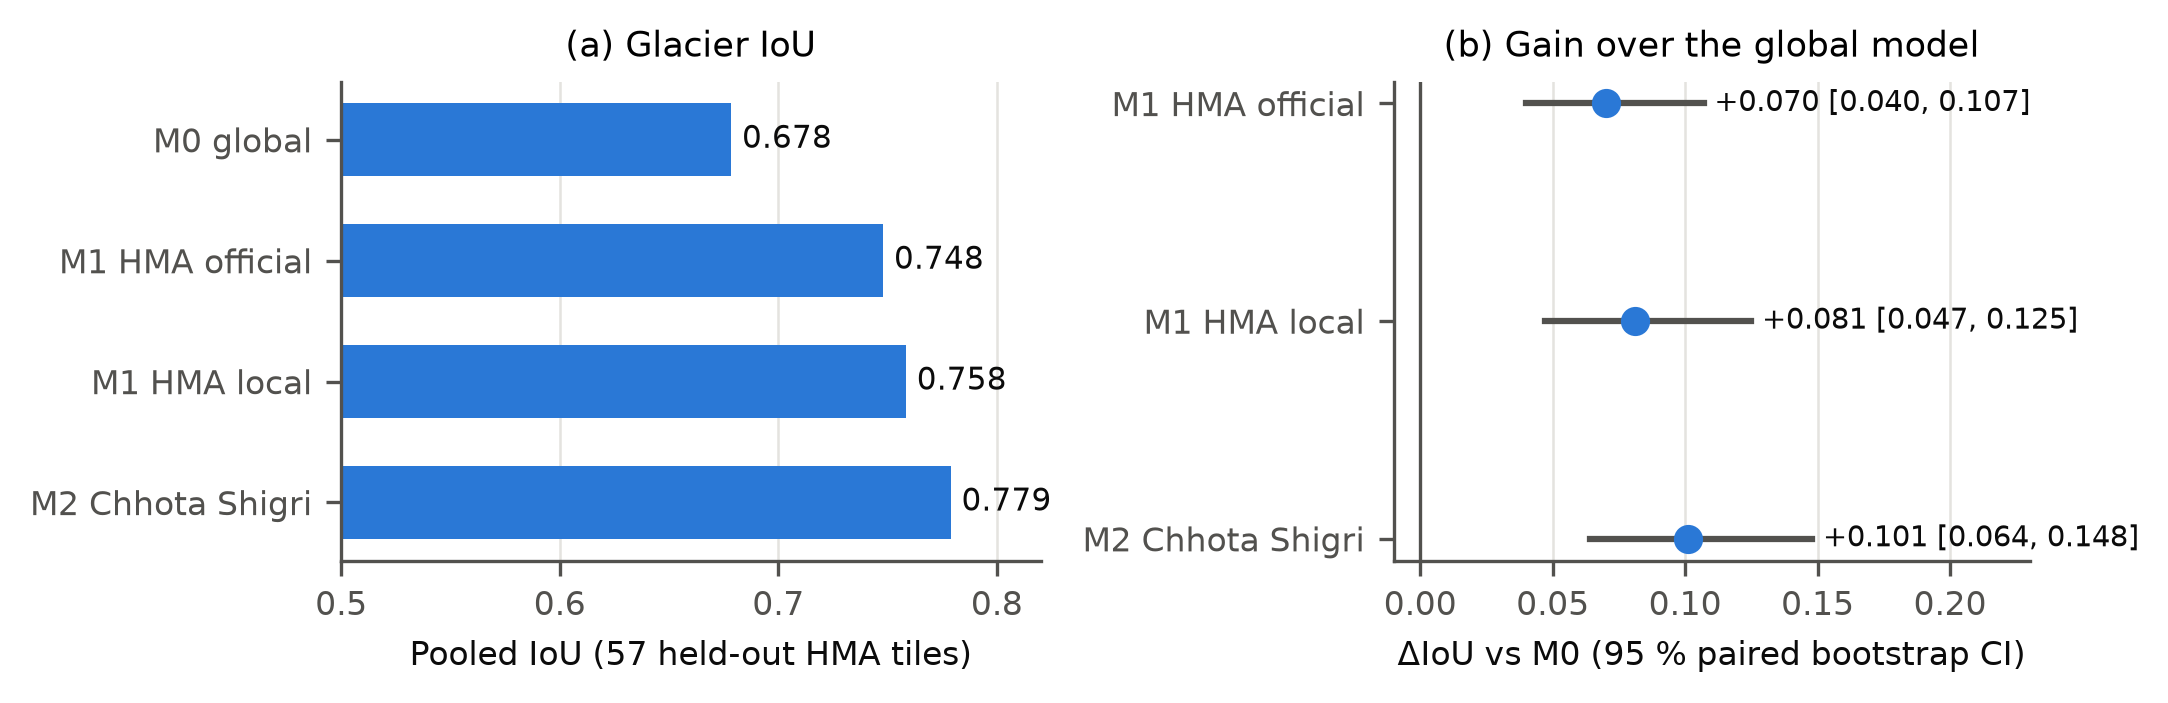
\includegraphics[width=\textwidth]{figures/fig_benchmark.png}
\caption{(a) Pooled glacier IoU on the 57 held-out HMA test tiles. (b) Gain over the global model M0 with 95\,\% confidence intervals from a paired bootstrap over tiles.}\label{fig:bench}
\end{figure}

On the 22 test tiles that contain SAR, with equal training budgets, adding the DEM to the optical bands raised the IoU from 0.676 to 0.824 ($+0.149$ [0.078, 0.241]), the largest effect in this study. Adding Sentinel-1 backscatter lowered it slightly, to 0.808 ($-0.016$ [$-0.029$, $-0.008$]); with a randomly initialised SAR branch and a short budget, SAR gave no benefit.

\subsection{Calibration and pseudo-labels}\label{subsec4.3}

Isotonic calibration reduced the held-out ECE of M1 from 0.239 to 0.011 (Fig.~\ref{fig:calib}), and of M0, M1-local, M2 and M3 from 0.225--0.234 to 0.016--0.053. The calibration showed that the raw outputs were strongly under-confident: a raw M1 probability of 0.70 corresponds to a glacier frequency of 0.97. Without calibration the consensus rule selected no pixel at all; with it, 292\,012 pixels were labelled glacier and 881\,732 background, and 34.7\,\% of the domain was left unlabelled (Fig.~\ref{fig:pl}). The unlabelled pixels are concentrated on the debris-covered margins, the terminus and the snow-affected tributary margins.

\begin{figure}[h]
\centering
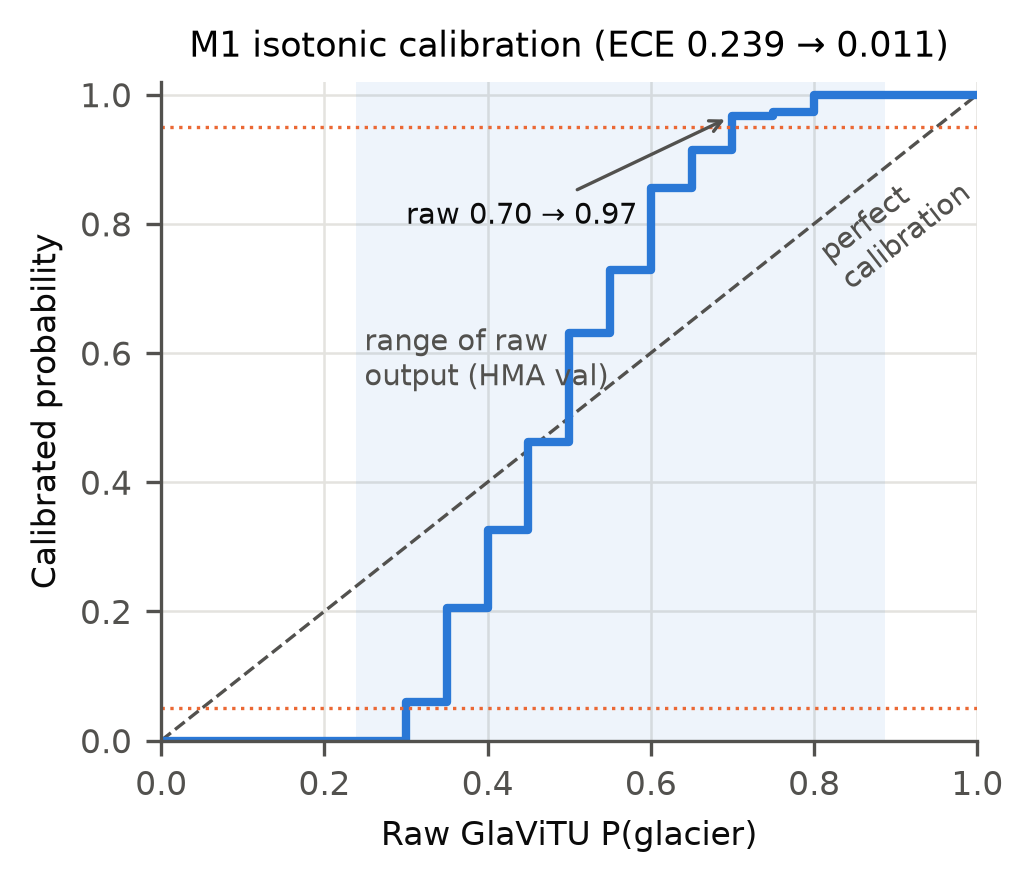
\includegraphics[width=0.55\textwidth]{figures/fig_calibration.png}
\caption{Isotonic calibration of M1, fitted on HMA validation tiles. The raw softmax output spans only 0.24--0.89 (shaded). Dotted lines: pseudo-label thresholds 0.05 and 0.95. ECE is computed on held-out tiles.}\label{fig:calib}
\end{figure}

\begin{figure}[h]
\centering
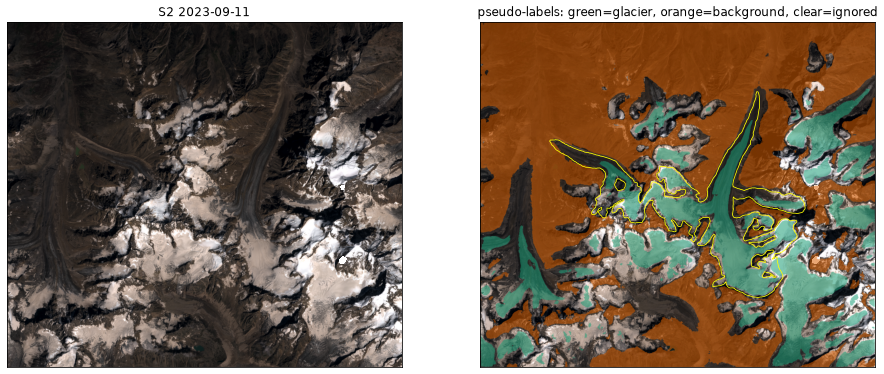
\includegraphics[width=\textwidth]{figures/pseudolabels_consensus.png}
\caption{Calibrated multi-temporal pseudo-labels. Left: Sentinel-2 scene of 11 September 2023 (true colour). Right: consensus labels from the even years 2018--2024 (green: glacier; orange: background; clear: unlabelled) with the RGI~7.0 outline (yellow).}\label{fig:pl}
\end{figure}

\subsection{Glacier outlines and area, 2017--2025}\label{subsec4.4}

The M2 outlines of the five analysis epochs are shown in Fig.~\ref{fig:outlines}. They agree closely along the clean-ice margins and differ mainly on the debris-covered tongue margins and the snow-affected tributary margins. Table~\ref{tab:epochs} gives the area of each epoch with its uncertainty budget. The multi-date ensemble reduced the between-scene area spread to 0.27--0.81\,\kmsq; single scenes in one season differ by up to about 1\,\kmsq\ because thin snow covers the debris-covered margins in some scenes and not in others. The threshold term is the largest component of the uncertainty in every year. The weakest epochs are 2017 and 2019, with two scenes each and more than 3\,\kmsq\ of the domain observed only once.

\begin{figure}[h]
\centering
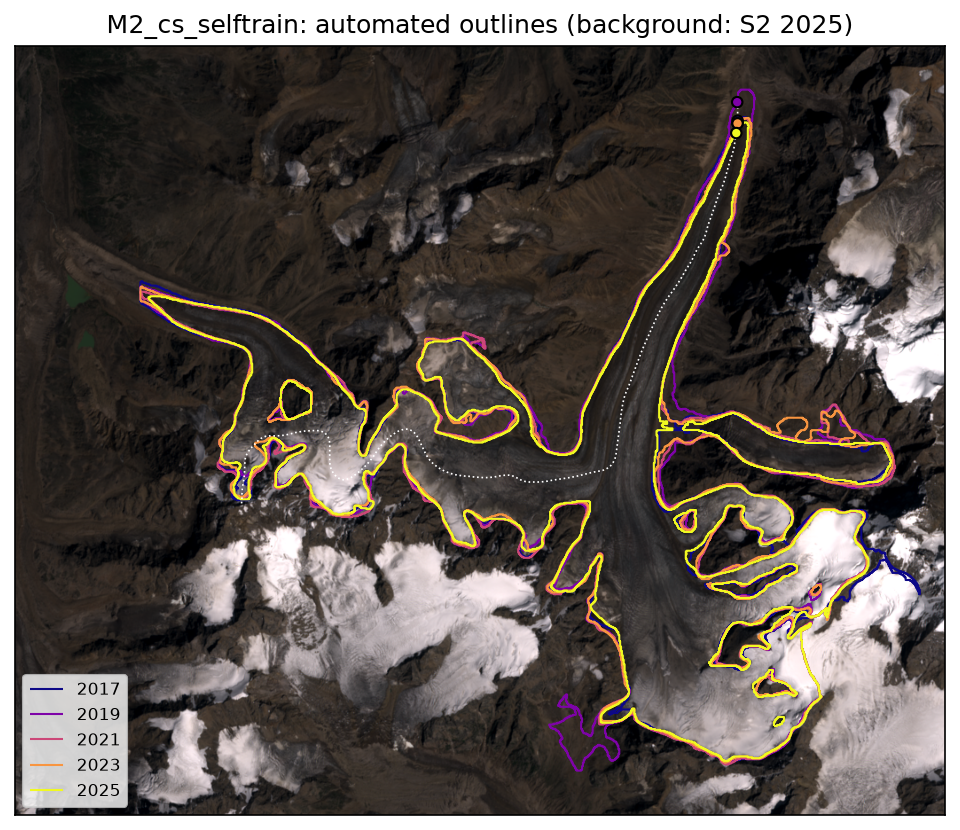
\includegraphics[width=0.85\textwidth]{figures/M2_cs_selftrain_yearly_outlines.png}
\caption{Automated M2 outlines of the analysis epochs 2017--2025 on the Sentinel-2 image of 2025. Dotted line: automatic centerline; dots: terminus positions.}\label{fig:outlines}
\end{figure}

\begin{table}[h]
\caption{Area of each analysis epoch: M2 with its uncertainty budget, and all models (\kmsq).}\label{tab:epochs}%
\begin{tabular*}{\textwidth}{@{\extracolsep\fill}lccccc}
\toprule
 & 2017 & 2019 & 2021 & 2023 & 2025 \\
\midrule
Scenes used & 2 & 2 & 2 & 6 & 2 \\
Area seen once (\kmsq) & 3.41 & 3.14 & 1.68 & 0.00 & 0.88 \\
\midrule
\textbf{M2 area} & \textbf{15.00} & \textbf{15.89} & \textbf{15.38} & \textbf{15.03} & \textbf{14.30} \\
$\sigma_\mathrm{buf}$ & 0.40 & 0.43 & 0.41 & 0.41 & 0.40 \\
$\sigma_\mathrm{thr}$ & 1.12 & 1.12 & 0.91 & 0.88 & 0.75 \\
$\sigma_\mathrm{surf}$ & 0.81 & 0.75 & 0.32 & 0.37 & 0.27 \\
$\sigma_A$ (Eq.~\ref{eq:sigmaA}) & 1.44 & 1.41 & 1.05 & 1.04 & 0.89 \\
\midrule
M0 global & 13.19 & 14.47 & 14.70 & 14.44 & 13.42 \\
M1 HMA official & 14.16 & 14.81 & 14.78 & 14.46 & 13.79 \\
M1-local & 14.42 & 15.43 & 15.24 & 15.26 & 14.10 \\
M3 HMA + SAR & 14.38 & 16.05 & 15.72 & 15.53 & 13.96 \\
Cross-model range & 1.80 & 1.59 & 1.03 & 1.09 & 0.88 \\
\midrule
Window 15 Aug--15 Oct (M1)\footnotemark[1] & 13.73 & 14.06 & 13.53 & 14.46 & 11.81 \\
\botrule
\end{tabular*}
\footnotetext{Published areas: 15.7\,\kmsq\ (c.~2003) \cite{wagnon2007} and 15.5\,\kmsq\ \cite{mandal2020}.}
\footnotetext[1]{Sensitivity run; later scenes include autumn snowfall and low sun.}
\end{table}

The weighted area trend over the analysis epochs is negative for every model but not significant for any (\kmsqa, 95\,\% confidence interval): M0 $-0.09$ [$-0.46$, 0.28], M1 $-0.18$ [$-0.38$, 0.02], M1-local $-0.02$ [$-0.32$, 0.27], M2 $-0.16$ [$-0.40$, 0.08] and M3 $-0.11$ [$-0.61$, 0.38]. For M2, the best-observed period 2021--2025 shows a loss of $-1.08 \pm 0.73$\,\kmsq\ ($-7.0$\,\%), which is also not significant at $2\sigma$. Including the even years (Fig.~\ref{fig:area}; Appendix~\ref{secA1}) does not change this conclusion. The 2017--2019 increase seen in all models coincides with the weakest epochs and is not interpreted as glacier growth.

Extending the window to 15 October lowered the area in four of five epochs, by up to 1.98\,\kmsq\ in 2025, lowered the mean agreement of M1 with the inventory (IoU 0.816 to 0.778), and created a spurious $-2.65$\,\kmsq\ step between 2023 and 2025. Late-season scenes map too little glacier because autumn snowfall and low sun hide the margins, which supports the choice of the core window.

\begin{figure}[h]
\centering
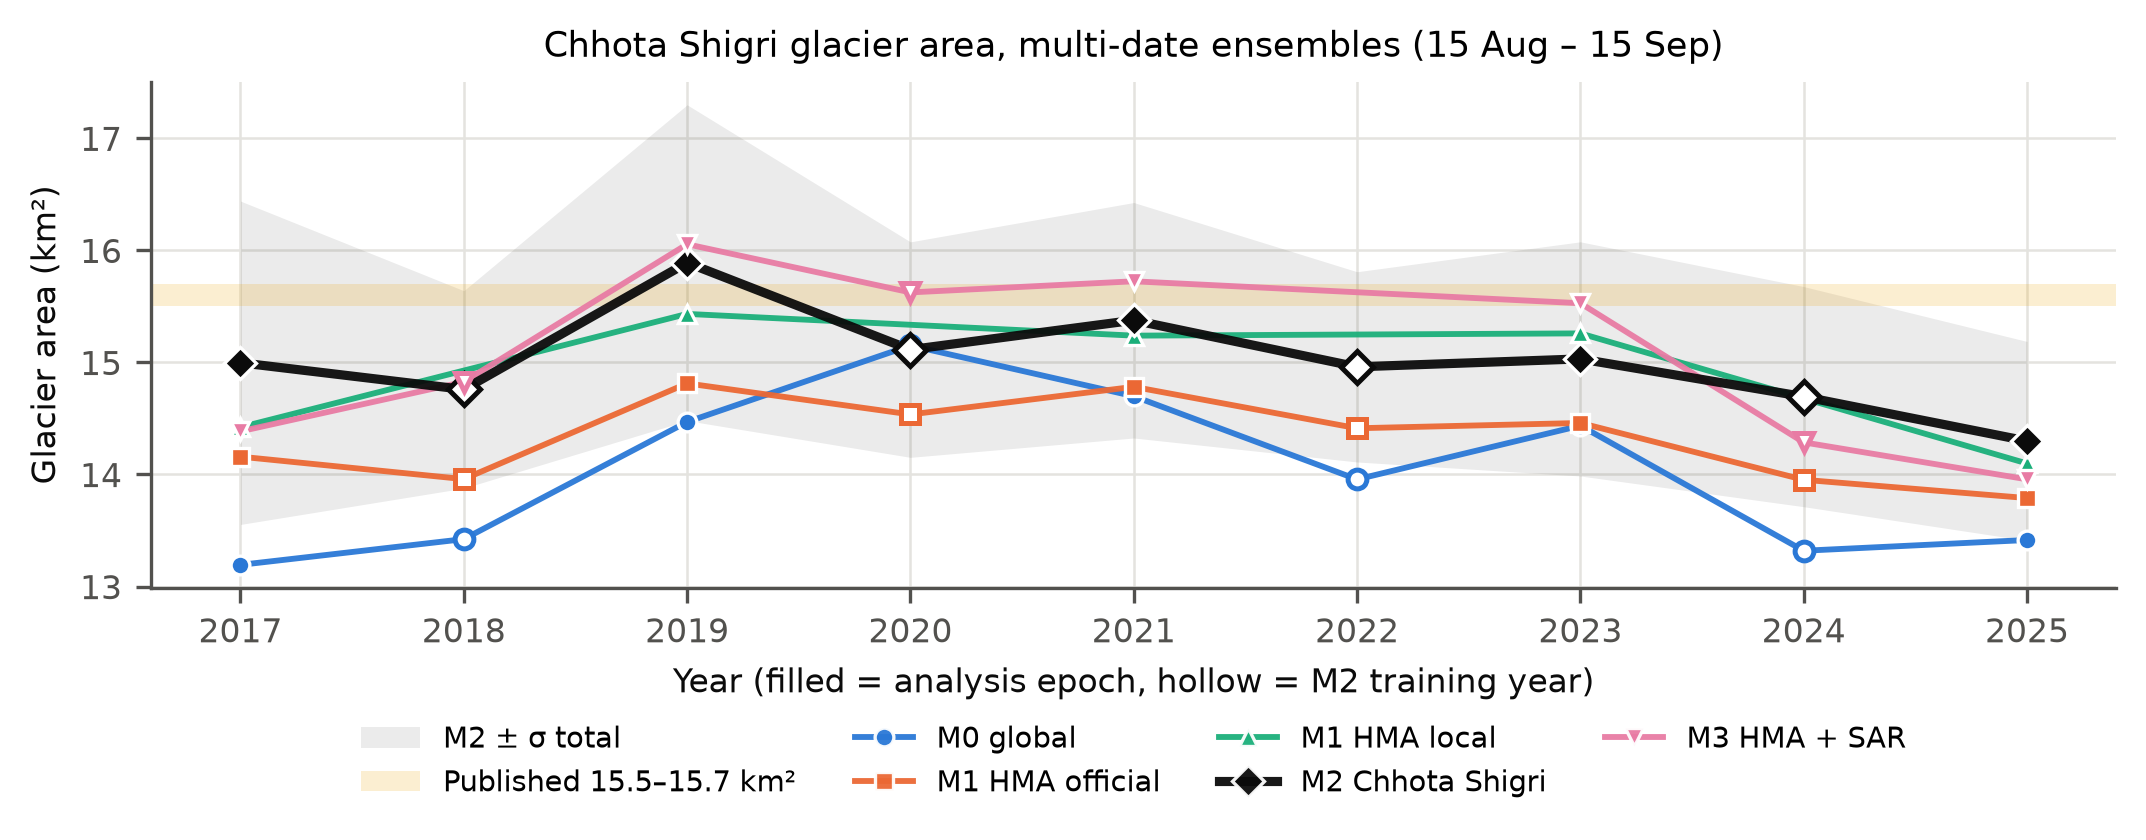
\includegraphics[width=\textwidth]{figures/fig_area_allyears.png}
\caption{Glacier area of all models for every year 2017--2025. Filled markers: analysis epochs; hollow markers: M2 training years (for M2 these values are not independent). Grey band: M2 $\pm\sigma_A$. Yellow band: published area.}\label{fig:area}
\end{figure}

\subsection{Terminus retreat}\label{subsec4.5}

Terminus change is the clearest signal (Table~\ref{tab:terminus}, Figs.~\ref{fig:terminus} and \ref{fig:zoom}). Over 2021--2025, all five models show retreat: 70--130\,m along the centerline (median 110\,m, about 28\,m\,a$^{-1}$) and 73--160\,m by the box method (median 80\,m, about 20\,m\,a$^{-1}$). Every value exceeds the measurement uncertainty of about 14\,m. Relative to 2017, all models place the 2025 terminus upstream (box method 17--498\,m). Periods that include 2017 or 2019 are inconsistent between models, because these epochs are the weakest. The absolute terminus position differs by up to about 800\,m between models on the debris-covered snout, so only changes are reported.

\begin{table}[h]
\caption{Terminus retreat by period across the five models (m; positive = retreat).}\label{tab:terminus}%
\begin{tabular*}{\textwidth}{@{\extracolsep\fill}lcccc}
\toprule
Period & Years & Centerline, median [min, max] & Box, median [min, max] & All retreat\footnotemark[1] \\
\midrule
2017--2019 & 2 & $-110$ [$-210$, 440] & $-100$ [$-218$, 465] & no \\
2019--2021 & 2 & 160 [$-110$, 240] & 105 [$-127$, 252] & no \\
2021--2023 & 2 & 0 [0, 40] & 5 [$-14$, 12] & no \\
2023--2025 & 2 & 100 [70, 110] & 80 [67, 148] & yes \\
\textbf{2021--2025} & \textbf{4} & \textbf{110 [70, 130]} & \textbf{80 [73, 160]} & \textbf{yes} \\
2019--2025 & 6 & 230 [20, 350] & 190 [33, 326] & yes \\
2017--2025 & 8 & 150 [10, 460] & 127 [17, 498] & yes \\
\botrule
\end{tabular*}
\footnotetext{Models: M0, M1, M1-local, M2, M3. Measurement uncertainty $\approx 14.2$--14.3\,m per period.}
\footnotetext[1]{All five models show retreat by the box method.}
\end{table}

\begin{figure}[h]
\centering
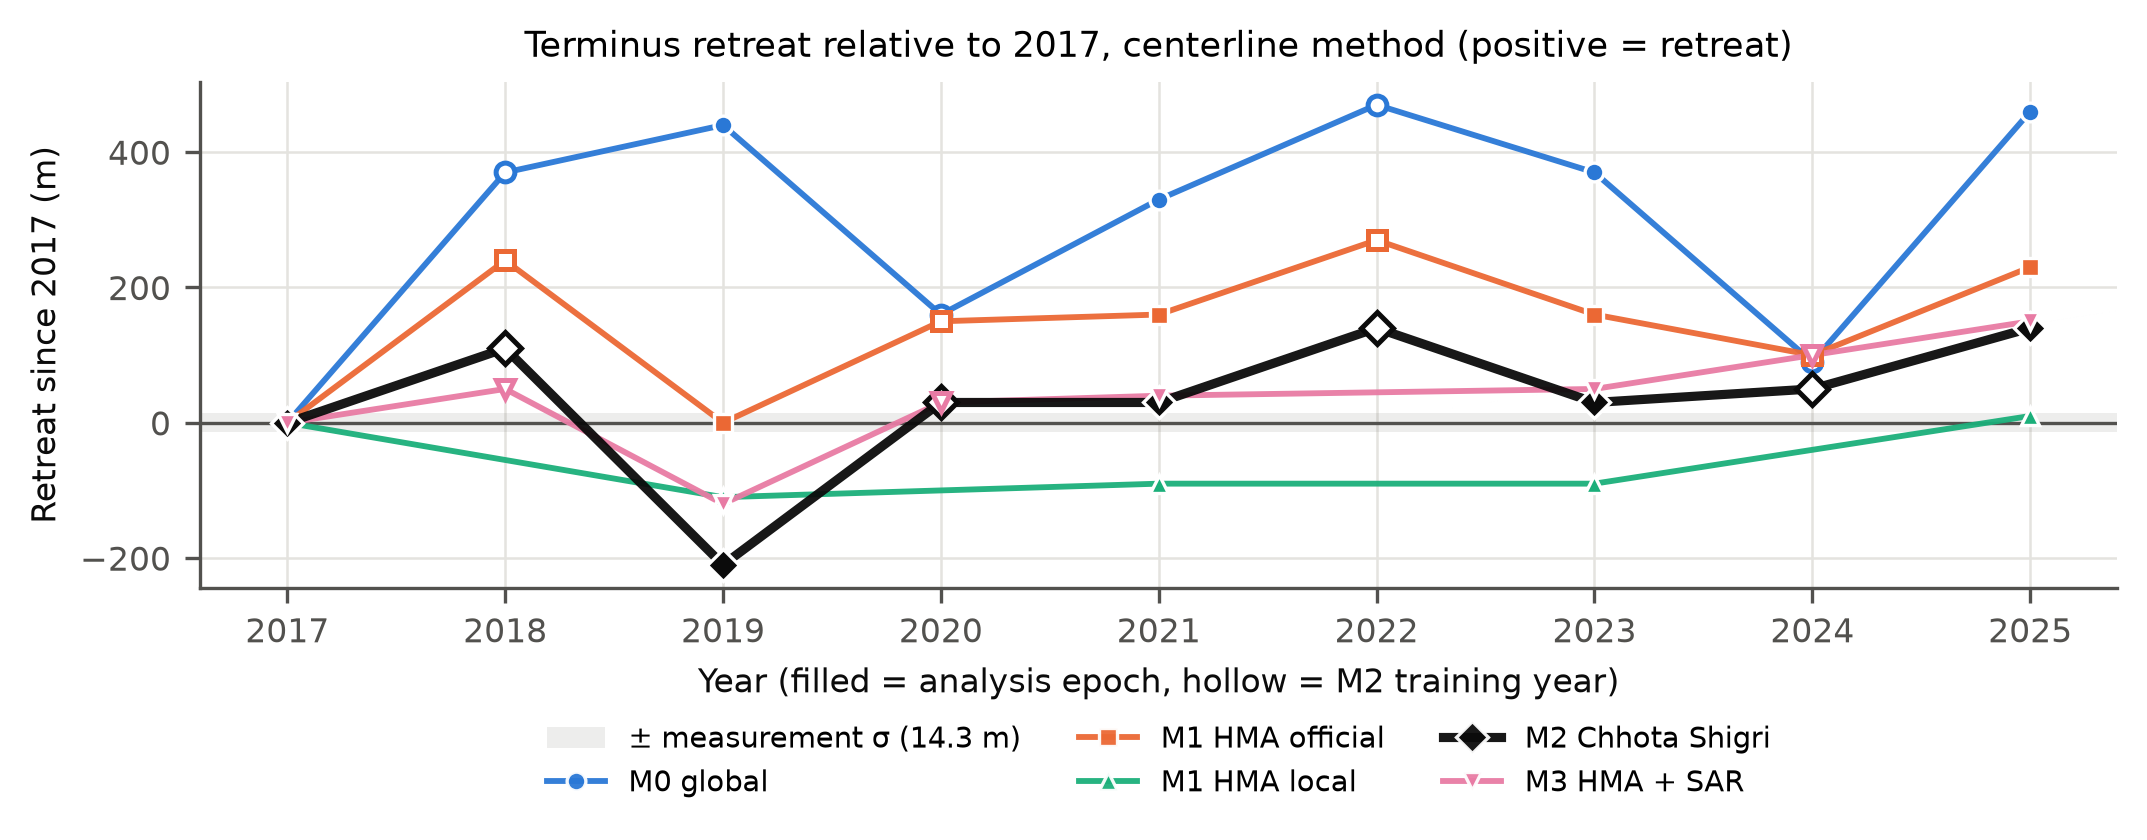
\includegraphics[width=\textwidth]{figures/fig_terminus_allyears.png}
\caption{Terminus retreat relative to 2017 along the centerline for all models and years. Grey band: $\pm$ measurement uncertainty. Hollow markers: M2 training years; even-year scenes were not co-registered.}\label{fig:terminus}
\end{figure}

\begin{figure}[h]
\centering
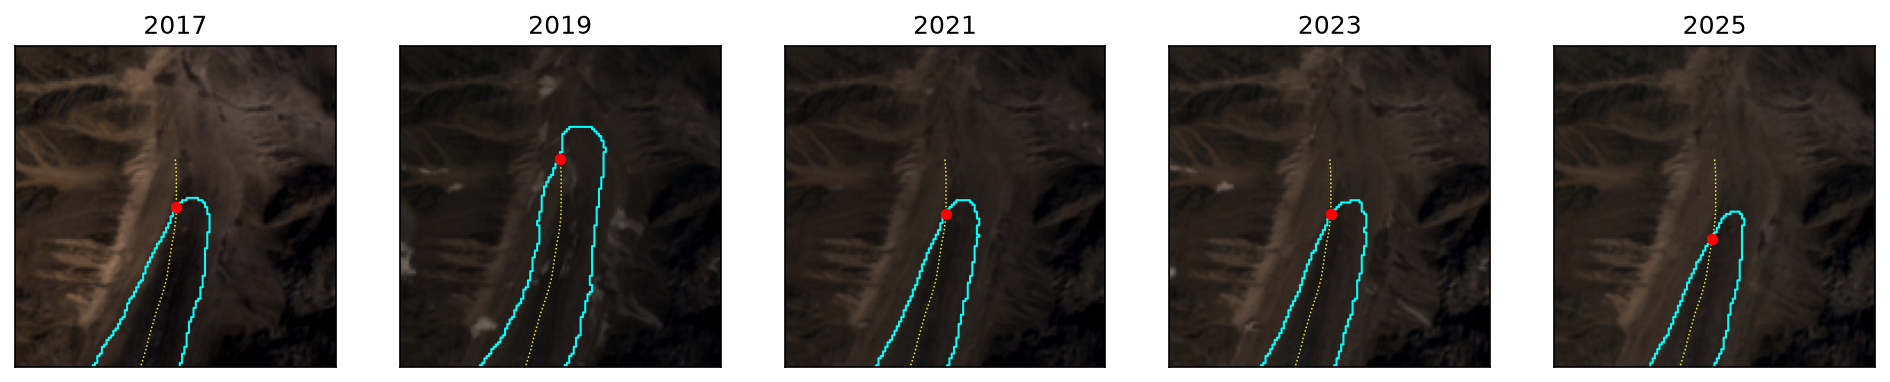
\includegraphics[width=\textwidth]{figures/M2_cs_selftrain_terminus_zoom.png}
\caption{Terminus of the M2 outlines (cyan) for each analysis epoch, with the centerline (yellow) and the measured terminus point (red).}\label{fig:zoom}
\end{figure}

\subsection{Spatial pattern of loss}\label{subsec4.6}

Over 2017--2025, M2 shows 0.94\,\kmsq\ of persistent loss against 1.74\,\kmsq\ of unstable margin pixels that were lost and re-appeared (Fig.~\ref{fig:yol}). Loss is strongly concentrated (Table~\ref{tab:patterns}, Fig.~\ref{fig:patterns}): within 250\,m of the terminus, 42\,\% of the baseline ice was lost, 6.7 times the glacier average, while the interior between 4900 and 5200\,m lost only 2--3\,\%. Loss is also enriched below 4500\,m and on slopes steeper than 40\textdegree. Hotspots of loss lie at the snout, at the tip of the north-western arm and along the eastern tributary margins (Fig.~\ref{fig:hotspots}). The descriptive logistic model separates lost from retained ice with a spatial-block cross-validated AUC of 0.94; among the terrain terms, steeper slope ($+0.47$, standardised coefficient), lower elevation ($-0.40$), north-facing aspect ($+0.29$) and proximity to the terminus ($-0.25$ for distance) favour loss. Aspect is confounded with the north-flowing tongue.

\begin{table}[h]
\caption{Where loss occurred (M2, 2017--2025).}\label{tab:patterns}%
\begin{tabular*}{\textwidth}{@{\extracolsep\fill}lcc}
\toprule
Terrain class & Loss fraction (\%) & Enrichment \\
\midrule
Within 250\,m of the terminus & 42 & 6.7 \\
250--1000\,m from the terminus & 22--23 & 3.4--3.5 \\
Elevation 4300--4500\,m & 28--33 & 4.4--5.1 \\
Slope $> 40$\textdegree & 36 & 5.6 \\
North-facing\footnotemark[1] & 17 & 2.7 \\
Interior, 4900--5200\,m & 2--3 & 0.4--0.5 \\
\botrule
\end{tabular*}
\footnotetext{Loss fraction: lost area divided by baseline area of the class. Enrichment: share of total loss divided by share of baseline area.}
\footnotetext[1]{Aspect is confounded with the north-flowing tongue.}
\end{table}

\begin{figure}[h]
\centering
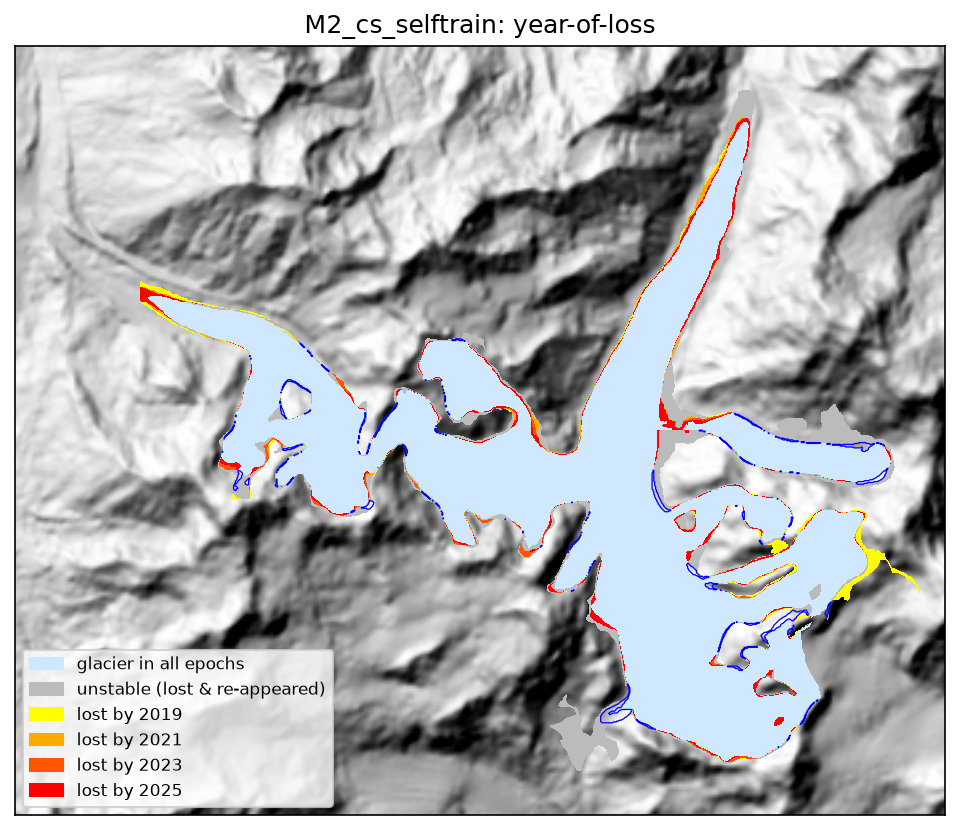
\includegraphics[width=0.75\textwidth]{figures/M2_cs_selftrain_year_of_loss.png}
\caption{Year of loss (M2). A pixel is assigned a loss year only if it is non-glacier in that and every later epoch; grey pixels were lost and re-appeared.}\label{fig:yol}
\end{figure}

\begin{figure}[h]
\centering
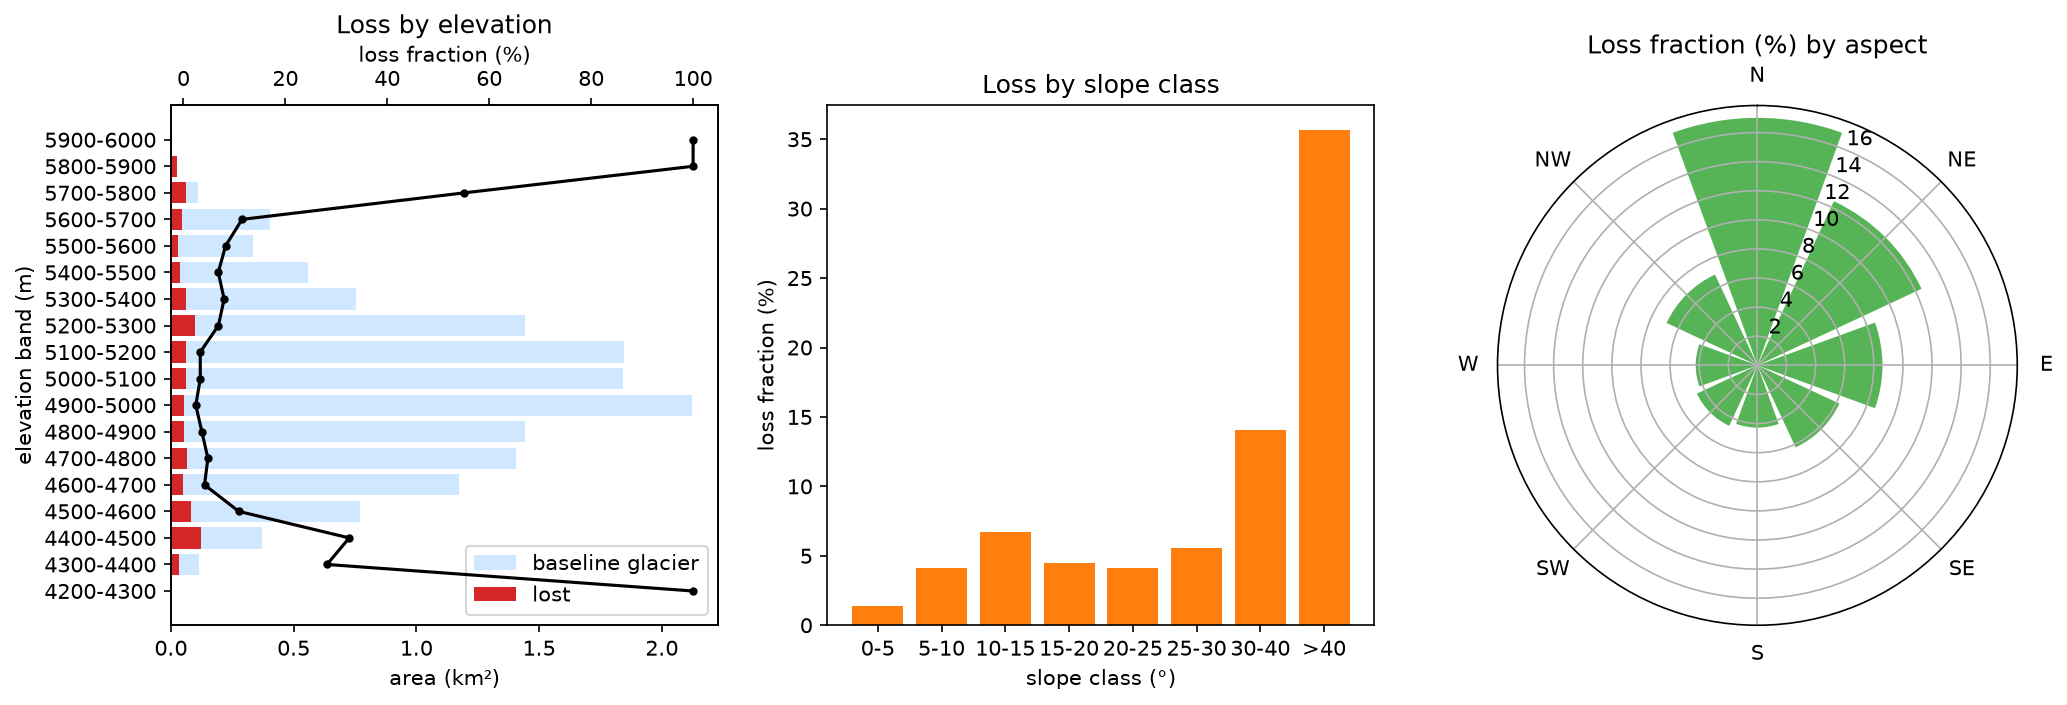
\includegraphics[width=\textwidth]{figures/M2_cs_selftrain_patterns.png}
\caption{Loss by elevation band (bars: baseline and lost area; line: loss fraction), by slope class and by aspect sector (M2, 2017--2025).}\label{fig:patterns}
\end{figure}

\begin{figure}[h]
\centering
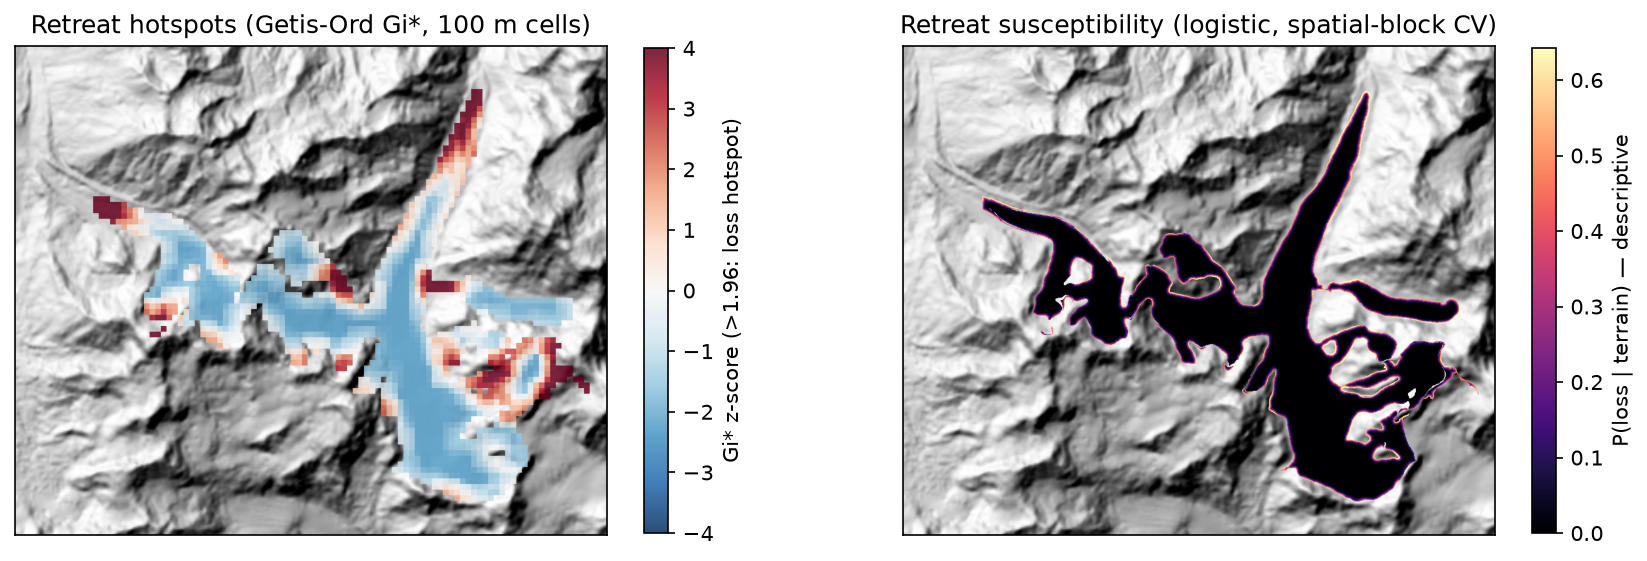
\includegraphics[width=\textwidth]{figures/M2_cs_selftrain_hotspots.png}
\caption{Left: Getis--Ord $G_i^*$ z-scores of loss on 100\,m cells ($z > 1.96$: hotspot). Right: descriptive logistic loss probability given terrain (spatial-block cross-validation). Neither is a forecast.}\label{fig:hotspots}
\end{figure}

\subsection{Agreement with inventory and published values}\label{subsec4.7}

Agreement with the 2002 RGI~7.0 outline was clearly higher for the site-adapted and regionally retrained models than for their teacher: M2 reached an IoU of 0.823--0.854 over the analysis epochs (mean 0.838), against 0.796--0.833 for M1 (mean 0.816), with a mean boundary distance of 43--52\,m against 58--68\,m. M1-local and M3 agreed about as well as M2 (mean IoU 0.836 and 0.838). Precision was at least 0.93 in every epoch, so the model rarely marks non-glacier as glacier; recall decreased from 0.883 in 2021 to 0.836 in 2025, consistent with a glacier that is smaller than its 2002 outline. The M2 areas (14.30--15.89\,\kmsq) are close to the published 15.5--15.7\,\kmsq\ \cite{wagnon2007,mandal2020}, and the retreat rate of about 20--28\,m\,a$^{-1}$ is lower than the long-term average implied by 800--850\,m of retreat over 1972--2009 \cite{gantayat2017}.

%%====================================================================%%
\section{Discussion}\label{sec5}
%%====================================================================%%

\subsection{Transfer and adaptation without manual labels}\label{subsec5.1}

The transfer hierarchy shows that a global glacier model can be adapted to a debris-affected region and then to a single glacier without drawing any outline. Regional fine-tuning gave the largest step, and it was reproduced with a small fraction of the original training budget on a laptop GPU. Site self-training added a further, significant gain on the regional test set. This gain cannot be attributed entirely to the site labels, because HMA tiles were replayed during self-training; on the site, M2 agrees better with the inventory than its teacher M1, but not better than M1-local or M3, so a site-specific accuracy gain cannot be demonstrated without independent contemporaneous outlines. The DEM was by far the most valuable input, in line with the difficulty of separating debris-covered ice from rock in optical bands \cite{scherler2011,xie2020}. That SAR did not help contrasts with the gains reported for the full GlaViTU training \cite{maslov2025}; the short budget and the randomly initialised SAR branch are the likely reasons, and the approximate $\sigma^0$ derived from terrain-corrected products differs from the benchmark input.

Calibration was a precondition for self-training. Label smoothing and the focal loss produce under-confident outputs \cite{guo2017}, so raw probabilities could not express confidence. Isotonic calibration on independent labelled tiles made the thresholds meaningful without using site data. Requiring agreement across scenes and across years left the changing margins unlabelled, so the pseudo-labels encode no assumption about change, and the alternating split of training and analysis years kept every measured epoch unseen.

\subsection{Detectability of area and terminus change}\label{subsec5.2}

The main limit on area change is not the model but the glacier surface. On the debris-covered margins, a thin snow cover appears and disappears within days, which changes single-scene area by about 1\,\kmsq. The multi-date median reduces this, but the remaining uncertainty of 0.9--1.4\,\kmsq\ per epoch is larger than the area change expected over eight years. Area change of this glacier is therefore not detectable at this precision, for any model. The terminus, in contrast, is a narrow feature measured along a fixed line, and its change of 70--160\,m over 2021--2025 is several times its measurement error and is reproduced by models with different training histories. Terminus position is therefore the more sensitive indicator for automated monitoring of a single glacier, while area change needs a longer period or more scenes per year.

\subsection{Limitations}\label{subsec5.3}

The 2017 and 2019 epochs rest on two scenes each, with more than 3\,\kmsq\ of the domain observed once, and the 2017 baseline needed the largest co-registration correction; all changes relative to 2017 inherit this weakness. Both 2025 scenes are from August, whereas 2023 extends to September, so part of the 2023--2025 change may be seasonal. The absolute terminus position on the debris-covered snout is uncertain by up to about 800\,m between models. Cloud shadow, terrain shadow and proglacial water are not masked explicitly. Even-year scenes were not co-registered, and the even-year results of M2 are not independent because M2 was trained on them. Finally, no contemporaneous independent outline exists for the site, so site accuracy is inferred from benchmark accuracy, agreement with an older inventory and temporal consistency.

%%====================================================================%%
\section{Conclusion}\label{sec6}
%%====================================================================%%

We showed that a published convolutional-transformer glacier model can be transferred to the Himalaya and adapted to Chhota Shigri Glacier with calibrated, multi-temporal pseudo-labels, without any manual outline. Regional fine-tuning and site self-training raised the held-out IoU from 0.678 to 0.779, and the DEM was the most important input. With a multi-date ensemble, the automated outlines are stable enough to detect terminus retreat of 70--160\,m (about 20--28\,m\,a$^{-1}$) over 2021--2025 in all five models, concentrated within 1\,km of the terminus, below 4500\,m and on steep margins. Area change over 2017--2025 is not detectable, because surface conditions on the debris-covered margins dominate the uncertainty. Future work should add more scenes per year, explicit shadow and water masks, and independent contemporaneous outlines, and should extend the approach to the glacial lakes that are relevant for GLOF risk.

\backmatter

\bmhead{Supplementary information}

The per-year tables for 2017--2025 relative to the 2017 baseline are given in Appendix~\ref{secA1}. % TODO(author): list any supplementary files.

\bmhead{Acknowledgements}

We thank K.~A.~Maslov and co-authors for publishing the GlaViTU code, weights and benchmark data, and the European Space Agency, the Copernicus programme, Microsoft Planetary Computer, Google Cloud, GLIMS and the RGI Consortium for open data. % TODO(author): add funding acknowledgements and a statement on the use of AI tools in preparing the manuscript, as required by the journal.

\section*{Declarations}

\begin{itemize}
\item \textbf{Funding:} TODO(author).
\item \textbf{Conflict of interest/Competing interests:} TODO(author).
\item \textbf{Ethics approval and consent to participate:} Not applicable.
\item \textbf{Consent for publication:} Not applicable.
\item \textbf{Data availability:} All input data are openly available: Sentinel-1 and Sentinel-2 (Copernicus), Copernicus DEM GLO-30 \cite{copdem}, RGI \cite{rgi6,rgi7}, GLIMS \cite{raup2007} and the GlaViTU benchmark \cite{maslov2024data}. Derived outlines and statistics: TODO(author).
\item \textbf{Materials availability:} Not applicable.
\item \textbf{Code availability:} The GlaViTU code is available from its authors \cite{maslov2025} (commit \texttt{8c4eead}). The processing code of this study: TODO(author).
\item \textbf{Author contribution:} TODO(author).
\end{itemize}

\begin{appendices}

\section{Year-by-year results relative to the 2017 baseline}\label{secA1}

This appendix extends the analysis to every year from 2017 to 2025, with 2017 as the baseline. Odd years are analysis epochs; even years were used to train M2, so M2 values for even years (marked $^\dagger$) are not independent: for example, the between-scene spread of M2 in 2018 is 0.04\,\kmsq\ against 0.55\,\kmsq\ for M1 on the same scenes. Even-year scenes were not co-registered, so their terminus uncertainty (pixel size only) is underestimated. Over all available years, the weighted area trend remains non-significant for every model (M0 $-0.145$ [$-0.384$, 0.094], M1 $-0.083$ [$-0.209$, 0.043], M2 $-0.064$ [$-0.181$, 0.052], M3 $-0.098$ [$-0.342$, 0.145]\,\kmsqa).

\begin{sidewaystable}
\caption{Data quality and M2 change relative to 2017 for every year.}\label{tab:a1}
\begin{tabular*}{\textheight}{@{\extracolsep\fill}lccccccccc}
\toprule
 & 2017 & 2018$^\dagger$ & 2019 & 2020$^\dagger$ & 2021 & 2022$^\dagger$ & 2023 & 2024$^\dagger$ & 2025 \\
\midrule
Scenes used & 2 & 3 & 2 & 4 & 2 & 4 & 6 & 2 & 2 \\
Mean clear looks per pixel & 1.90 & 2.79 & 1.91 & 3.91 & 1.96 & 3.82 & 5.27 & 1.88 & 1.98 \\
Area seen once (\kmsq) & 3.41 & 0.57 & 3.14 & 0.00 & 1.68 & 0.03 & 0.00 & 5.64 & 0.88 \\
Co-registration residual (m) & 1.41 & -- & 1.41 & -- & 0.71 & -- & 1.41 & -- & 1.58 \\
\midrule
Area (\kmsq) & 15.00 & 14.76 & 15.89 & 15.11 & 15.38 & 14.96 & 15.03 & 14.69 & 14.30 \\
$\sigma_A$ (\kmsq) & 1.44 & 0.88 & 1.41 & 0.96 & 1.05 & 0.85 & 1.04 & 0.98 & 0.89 \\
$\sigma_\mathrm{surf}$ (\kmsq) & 0.81 & 0.04 & 0.75 & 0.07 & 0.32 & 0.13 & 0.37 & 0.37 & 0.27 \\
$\Delta A$ from 2017 (\kmsq) & 0 & $-0.24$ & $+0.89$ & $+0.12$ & $+0.38$ & $-0.04$ & $+0.03$ & $-0.30$ & $-0.70$ \\
$\sigma_{\Delta A}$ (\kmsq) & -- & 1.05 & 1.25 & 1.03 & 1.07 & 1.07 & 1.09 & 1.11 & 1.09 \\
$\Delta A$ from 2017 (\%) & 0 & $-1.6$ & $+6.0$ & $+0.8$ & $+2.5$ & $-0.2$ & $+0.2$ & $-2.0$ & $-4.7$ \\
Lost since 2017 (\kmsq) & -- & 0.61 & 0.50 & 0.49 & 0.51 & 0.54 & 0.66 & 0.74 & 0.94 \\
Gained since 2017 (\kmsq) & -- & 0.37 & 1.40 & 0.60 & 0.89 & 0.51 & 0.70 & 0.44 & 0.24 \\
Retreat since 2017, centerline (m) & 0 & 110 & $-210$ & 30 & 30 & 140 & 30 & 50 & 140 \\
Retreat since 2017, box (m) & 0 & 83 & $-218$ & 47 & 35 & 111 & 41 & 49 & 108 \\
\botrule
\end{tabular*}
\footnotetext{No area change is significant at $2\sigma$. 2022: one scene rejected as an area outlier. 2024: one scene contained no valid data. Co-registration was not run for even years.}
\end{sidewaystable}

\begin{sidewaystable}
\caption{Area change and terminus retreat relative to 2017 for all models and years.}\label{tab:a2}
\setlength{\tabcolsep}{4pt}%
\begin{tabular*}{\textheight}{@{\extracolsep\fill}lcccccccc}
\toprule
 & 2018 & 2019 & 2020 & 2021 & 2022 & 2023 & 2024 & 2025 \\
\midrule
\multicolumn{9}{@{}l}{\textit{$\Delta A$ from 2017 (\kmsq)}} \\
M0 global & $+0.23$ & $+1.28$ & $+1.96$ & $+1.51$ & $+0.76$ & $+1.24$ & $+0.13$ & $+0.22$ \\
M1 HMA official & $-0.20$ & $+0.65$ & $+0.38$ & $+0.62$ & $+0.25$ & $+0.30$ & $-0.21$ & $-0.37$ \\
M1-local & -- & $+1.01$ & -- & $+0.82$ & -- & $+0.84$ & -- & $-0.32$ \\
M2 Chhota Shigri & $-0.24^\dagger$ & $+0.89$ & $+0.12^\dagger$ & $+0.38$ & $-0.04^\dagger$ & $+0.03$ & $-0.30^\dagger$ & $-0.70$ \\
M3 HMA + SAR & $+0.44$ & $+1.67$ & $+1.24$ & $+1.34$ & -- & $+1.14$ & $-0.10$ & $-0.43$ \\
\midrule
\multicolumn{9}{@{}l}{\textit{Retreat since 2017, box method (m)}} \\
M0 global & 386 & 465 & 203 & 338 & 501 & 350 & 144 & 498 \\
M1 HMA official & 250 & 71 & 147 & 176 & 290 & 161 & 110 & 260 \\
M1-local & -- & $-100$ & -- & $-56$ & -- & $-51$ & -- & 17 \\
M2 Chhota Shigri & $83^\dagger$ & $-218$ & $47^\dagger$ & 35 & $111^\dagger$ & 41 & $49^\dagger$ & 108 \\
M3 HMA + SAR & 65 & $-126$ & 31 & 47 & -- & 47 & 97 & 127 \\
Median [min, max] & 167 [65, 386] & $-100$ [$-218$, 465] & 97 [31, 203] & 47 [$-56$, 338] & 290 [111, 501] & 47 [$-51$, 350] & 104 [49, 144] & 127 [17, 498] \\
\botrule
\end{tabular*}
\footnotetext{M1-local was run on the analysis epochs only; M3 has no 2022 result (no Sentinel-1 composite). The set of models therefore differs between odd and even years.}
\end{sidewaystable}

\end{appendices}

\bibliography{references}

\end{document}
